
% \documentclass[12pt,a4paper]{article}
% \usepackage{ragged2e}
% \usepackage{graphicx} % Required for insert
% \usepackage{geometry}
% \geometry{
%     a4paper,
%     left=20mm,
%     right=20mm,
%     top=20mm,
%     bottom=20mm
% }

% \begin{document}

% \begin{titlepage}
    
% \begin{center}
\vspace{8pt}
\Large\textbf{RAJIV GANDHI INSTITUTE OF TECHNOLOGY}\\
\vspace{8pt}
\Large\textbf{GOVERNMENT ENGINEERING COLLEGE}\\
\vspace{8pt}
\Large\textbf{KOTTAYAM-686 501}\\
\vspace{8pt}
\begin{center}

\includegraphics[scale=0.25]{rit.jpg}
\end{center}
\normalsize \textbf{DEPARTMENT OF \\ COMPUTER SCIENCE AND ENGINEERING} \\
\vspace{10pt}
\Large{CSD 334 MINI PROJECT REPORT}\\ \vspace{15pt}
\Large {\textsc{\textbf{FastTrack}}}\\
\vspace{20pt}
\large \textbf{Report Submitted by }\\
\vspace{10pt}
\large {\textbf{Jessin Sunny (Reg. No: KTE22CS036)}}\\
\large {\textbf{Akhil S Nair (Reg. No: KTE22CS009) }}\\
\large {\textbf{Alwin Philip (Reg. No: KTE22CS012)}}\\
\large {\textbf{Edwin Varkey (Reg. No: KTE22CS028)}}\\
\begin{center}

\includegraphics[scale=0.25]{ktu.jpg}
\end{center}
\fontsize{18pt}{12pt}\selectfont {APJ ABDUL KALAM TECHNOLOGICAL UNIVERSITY\vspace{5pt} THIRUVANANTHAPURAM}
\\\vspace{10pt}
\normalsize {APRIL 2025}
\end{center}

% \end{titlepage}

% \newpage
\thispagestyle{empty}
\begin{center}
\Large\textbf{RAJIV GANDHI INSTITUTE OF TECHNOLOGY}
\vspace{10pt}
\\
\Large\textbf{GOVERNMENT ENGINEERING COLLEGE}\\
\vspace{10pt}
\Large\textbf{KOTTAYAM-686 501}\\
\vspace{10pt}
\begin{center}

\includegraphics[scale=0.25]{rit.jpg}
\end{center}
\vspace{5 pt}

\Large \textbf{DEPARTMENT OF \\COMPUTER SCIENCE AND ENGINEERING} 
\\
\vspace{50 pt}
\Large \textbf{Vision of the Department }\\
\vspace{10pt}
\normalsize{To be a centre of excellence for inclusively nurturing young minds to become innovative computing professionals committed to sustainable development and societal empowerment.}

\vspace{40 pt}

\Large \textbf{Mission of the Department }\\
\vspace{10pt}
\normalsize{
\begin{itemize}
\item{To offer a solid foundation in computing and technology for crafting competent professionals.}
\item{To promote innovative and entrepreneurial skills of students by exposing them to the forefront of developments in the field of computing.}
\item{To inculcate strong ethical values in the young minds to work with commitment for the progress of the nation.}
\end{itemize}
}


\end{center}
% \newpage
\thispagestyle{empty}
\begin{center}
\Large\textbf{RAJIV GANDHI INSTITUTE OF TECHNOLOGY}
\vspace{10pt}
\\
\Large\textbf{GOVERNMENT ENGINEERING COLLEGE}\\
\vspace{10pt}
\Large\textbf{KOTTAYAM-686 501}\\
\vspace{20pt}
\begin{center}

\includegraphics[scale=0.25]{rit.jpg}
\end{center}
\large \textbf{DEPARTMENT OF \\ COMPUTER SCIENCE AND ENGINEERING} 
\\
\vspace{20 pt}
\linespread{1.5}
\Large \textbf{CERTIFICATE}\\
\vspace{20 pt}
\justifying
\normalsize{\emph{\hspace{10pt}{This is to certify that this report entitled \textbf{\textsc{FastTrack}} is an authentic report of the project done by \textbf{Jessin Sunny (Reg. No: KTE22CS036), Akhil S Nair (Reg. No: KTE22CS009), Alwin Philip (Reg. No: KTE22CS012) and  Edwin Varkey (Reg. No: KTE22CS028)} during the academic year \textbf{2024-25}, in partial fulfillment of the requirements for the award of the Degree of Bachelor of Technology in Computer Science and Engineering of APJ Abdul Kalam Technological University, Thiruvananthapuram.}}}
\vspace{45pt}
\begin{center}
\begin{tabular}{l r}
{GUIDE} & \hspace{310pt}{COORDINATOR}
\end{tabular}
\end{center}
\vspace{45pt}
\begin{center}
HEAD OF THE DEPARTMENT
\end{center}

\end{center}
% \newpage
\thispagestyle{empty}
\chapter*{\centering Acknowledgement \centering}
\addcontentsline{toc}{chapter}{\numberline{}Acknowledgement}%
Every successful project is a result of dedication, hard work, and the invaluable support of many individuals. We sincerely appreciate the guidance, encouragement, and contributions of everyone who played a role in making this project a success.
\\
 We express our sincere gratitude to \textbf{Dr. Prince A., Principal, RIT Kottayam} for making the resources available at the right time without which this project would not have been a success.
 \\
We take this opportunity to express a deep sense of gratitude to \textbf{Prof. Kavitha N., Associate Professor \& Head, Department of Computer Science and Engineering}.
\\
 We also take this opportunity to express our profound gratitude and deep regards to our guide \textbf{Prof. Anu Bonia Francis, Assistant Professor} for her exemplary guidance, monitoring and constant encouragement throughout the course of this project. The blessing, help and guidance given by her from time to time shall carry us a long way in the journey of life on which we are about to embark.
 \\
 We also express our gratitude to Project Coordinators \textbf{Prof. Anu Bonia Francis, Assistant Professor} and \textbf{Dr. Raji R. Pillai} for the cordial support, valuable information and guidance, which helped us in completing this task through various stages.
 \\
 We would also like to express our gratitude to \textbf{teaching} and \textbf{non-teaching staffs} for providing us with the necessary facilities and support during our Mini Project hours, which greatly contributed to the completion of our project
 \\
 Last, but not least, we thank \textbf{almighty}, \textbf{our parents} and \textbf{friends} for their constant encouragement without which this project would not have been possible.
 \\
\vspace{40pt}
\begin{FlushRight}
Jessin Sunny
\\Akhil S Nair
\\Alwin Philip
\\Edwin Varkey
\end{FlushRight}
% \newpage



% \end{document}


\documentclass[12 pt,a4paper]{report}
%---------------------------------------Including the various packages----------------------
\usepackage{amssymb}
\usepackage{graphicx}
\usepackage{amsmath,bm}
\usepackage[toc,page]{appendix}
\usepackage{setspace}
\usepackage{amsthm}
\usepackage{amsfonts}
\usepackage{float}
\usepackage{url}
\usepackage{mathtools}
\usepackage{varwidth}
\usepackage{algorithm2e}
\usepackage[skip=10pt]{subcaption}
\usepackage{sidecap}
\usepackage{caption}
\usepackage{enumitem}
\usepackage[classfont=bold,
            langfont=roman,
            funcfont=italic]{complexity}
\usepackage{cite}
\usepackage[none]{hyphenat}
\usepackage{breqn}
\usepackage{array}
\usepackage{tikz}
\usepackage{regexpatch}
\usepackage[section]{placeins}
\usepackage{float}
\usepackage{lipsum}
\usepackage{regexpatch}
\usepackage{makeidx}
\usepackage{setspace}
\usepackage{array}
\usepackage[left=2cm,top=1in,right=2cm,bottom=1in,bindingoffset=0.4cm]{geometry}

\usepackage{fancyhdr} 
\usepackage{ragged2e}
\usepackage{algorithm2e}
\usepackage{rotating}
\usepackage{titlesec}
\usepackage{afterpage}
\usepackage{fancyvrb}
\usepackage[T1]{fontenc}
\usetikzlibrary{decorations.pathmorphing}
\usepackage{pgfplots}
\usepackage{longtable}
%\usepackage{hyperref}
%\urlstyle{same}
\captionsetup[figure]{width=0.9\linewidth}
%---------------------------------Redefining existing commands-------------------------------
\makeatletter
\renewcommand{\headrulewidth}{0pt}
\renewcommand\bibname{References}
\renewcommand{\@algocf@capt@plain}{above}
\renewcommand{\chaptermark}[1]{\markboth{#1}{}}
\xpatchcmd{\chaptermark}{\MakeUppercase}{}{}{}
\xpatchcmd{\sectionmark}{\MakeUppercase}{}{}{}
\xpatchcmd*{\tableofcontents}{\MakeUppercase}{}{}{}
% \renewcommand{\listfigurename}{List of Figures and Algorithms}
%------------------------------Setting different Counters and lengths--------------------------------
\makeatother
\setcounter{secnumdepth}{4}
\setcounter{chapter}{0}
\setcounter{tocdepth}{4}
\setlength{\headheight}{14.5pt}
\setlength\extrarowheight{5pt}
\setlength{\textfloatsep}{5pt}
%-------------------------------Defining new commands -----------------------------------------------
\makeatletter
\newfloat{Algorithm}{luc}{Algorithm}[chapter]
\newtheorem{theorem}{Theorem}[section]
\newtheorem{remark}{Remark}[section]
\newtheorem{definition}{Definition}[section]
\newtheorem{lemma}{Lemma}[section]
\newtheorem{corollary}{Corollary}[section]
\newtheorem{example}{Example}[section]
\newtheorem{fact}{Fact}[section]
\newtheorem{facts}{Facts}[section]
\newtheorem*{claim}{Claim}
\newtheorem*{result}{Result}
\newtheorem*{remarks}{Remarks}
\newcommand{\norm}[1]{\left\lVert#1\right\rVert}
\newcommand{\ie}{\textit{i}.\textit{e}.}
\newcommand\blankpage{
    \null
    \thispagestyle{empty}
    \addtocounter{page}{-2}
    \newpage
    \cleardoublepage
    }
\newcolumntype{L}{>{\centering\arraybackslash}m{14cm}}
\newcolumntype{M}{>{\centering\arraybackslash}m{15cm}}
\DeclarePairedDelimiter\ceil{\lceil}{\rceil}
\DeclarePairedDelimiter\floor{\lfloor}{\rfloor}
\makeatother
%-------------------------------Fancy Styles, Headers,Footers,Page Numbers etc-----------------------------------
\fancyhf{}
\fancyhead[R]
{
   \itshape
   \ifnum\value{chapter}>0 \chaptername\ \thechapter. \fi
   \leftmark
}
\fancyfoot[C]{\thepage}
\fancyfoot[L]{\emph{Dept of CSE-RIT-Kottayam}}
\fancypagestyle{plain}
{
  \renewcommand{\headrulewidth}{0pt}
  \fancyhf{}
  \fancyfoot[C]{\thepage}
}
%-----------------------------------Changing the font size of sections, subsections etc------------------------
\titleformat*{\section}{\LARGE\bfseries}
\titleformat*{\subsection}{\Large\bfseries}
\titleformat*{\subsubsection}{\large\bfseries}
%\titleformat*{\paragraph}{\large\bfseries}
%\titleformat*{\subparagraph}{\large\bfseries}
%-----------------------------Other settings ---------------------------------------------------------
\makeatletter
\def\verbatim@font{\normalfont}% select the font
%\let\do\do@noligs
%\verbatim@nolig@list}
%\makeatother
\def\Verbatim@nolig@list{\do\`\do\<\do\>\do\,\do\'\do\-\do\{\do\}}
\titleformat{\chapter}[display]
{\normalfont\huge\bfseries\centering}{\chaptertitlename\ \thechapter}{20pt}{\Huge}
\titlespacing*{\chapter}{0pt}{-40pt}{20pt}
\lineskiplimit=-1pt\relax
\hyphenation{thatshouldnot}
\makeindex
\pagestyle{fancy} 
\sloppy
%------------------------------------------------------------------------------------------------------
\begin{document}
%--------------------------Here starts the document--------------------------------------------------
\RestyleAlgo{boxruled}
\LinesNumbered
\thispagestyle{empty}
\pagenumbering{gobble}
\onehalfspacing
%--------------------------Here include the cover page----------------------------------
\begin{center}
\vspace{8pt}
\Large\textbf{RAJIV GANDHI INSTITUTE OF TECHNOLOGY}\\
\vspace{8pt}
\Large\textbf{GOVERNMENT ENGINEERING COLLEGE}\\
\vspace{8pt}
\Large\textbf{KOTTAYAM-686 501}\\
\vspace{8pt}
\begin{center}

\includegraphics[scale=0.25]{rit.jpg}
\end{center}
\normalsize \textbf{DEPARTMENT OF \\ COMPUTER SCIENCE AND ENGINEERING} \\
\vspace{10pt}
\Large{CSD 334 MINI PROJECT REPORT}\\ \vspace{15pt}
\Large {\textsc{\textbf{FastTrack}}}\\
\vspace{20pt}
\large \textbf{Report Submitted by }\\
\vspace{10pt}
\large {\textbf{Jessin Sunny (Reg. No: KTE22CS036)}}\\
\large {\textbf{Akhil S Nair (Reg. No: KTE22CS009) }}\\
\large {\textbf{Alwin Philip (Reg. No: KTE22CS012)}}\\
\large {\textbf{Edwin Varkey (Reg. No: KTE22CS028)}}\\
\begin{center}

\includegraphics[scale=0.25]{ktu.jpg}
\end{center}
\fontsize{18pt}{12pt}\selectfont {APJ ABDUL KALAM TECHNOLOGICAL UNIVERSITY\vspace{5pt} THIRUVANANTHAPURAM}
\\\vspace{10pt}
\normalsize {APRIL 2025}
\end{center}
\newpage
%--------------------------Here include the dept mission and vision----------------------------------
\newpage
\thispagestyle{empty}
\begin{center}
\Large\textbf{RAJIV GANDHI INSTITUTE OF TECHNOLOGY}
\vspace{10pt}
\\
\Large\textbf{GOVERNMENT ENGINEERING COLLEGE}\\
\vspace{10pt}
\Large\textbf{KOTTAYAM-686 501}\\
\vspace{10pt}
\begin{center}

\includegraphics[scale=0.25]{rit.jpg}
\end{center}
\vspace{5 pt}

\Large \textbf{DEPARTMENT OF \\COMPUTER SCIENCE AND ENGINEERING} 
\\
\vspace{50 pt}
\Large \textbf{Vision of the Department }\\
\vspace{10pt}
\normalsize{To be a centre of excellence for inclusively nurturing young minds to become innovative computing professionals committed to sustainable development and societal empowerment.}

\vspace{40 pt}

\Large \textbf{Mission of the Department }\\
\vspace{10pt}
\normalsize{
\begin{itemize}
\item{To offer a solid foundation in computing and technology for crafting competent professionals.}
\item{To promote innovative and entrepreneurial skills of students by exposing them to the forefront of developments in the field of computing.}
\item{To inculcate strong ethical values in the young minds to work with commitment for the progress of the nation.}
\end{itemize}
}


\end{center}
\newpage

%--------------------------Here include the certificate----------------------------------

\newpage
\thispagestyle{empty}
\begin{center}
\Large\textbf{RAJIV GANDHI INSTITUTE OF TECHNOLOGY}
\vspace{10pt}
\\
\Large\textbf{GOVERNMENT ENGINEERING COLLEGE}\\
\vspace{10pt}
\Large\textbf{KOTTAYAM-686 501}\\
\vspace{20pt}
\begin{center}

\includegraphics[scale=0.25]{rit.jpg}
\end{center}
\large \textbf{DEPARTMENT OF \\ COMPUTER SCIENCE AND ENGINEERING} 
\\
\vspace{20 pt}
\linespread{1.5}
\Large \textbf{CERTIFICATE}\\
\vspace{20 pt}
\justifying
\normalsize{\emph{\hspace{10pt}{This is to certify that this report entitled \textbf{\textsc{FastTrack}} is an authentic report of the project done by \textbf{Jessin Sunny (Reg. No: KTE22CS036), Akhil S Nair (Reg. No: KTE22CS009), Alwin Philip (Reg. No: KTE22CS012) and  Edwin Varkey (Reg. No: KTE22CS028)} during the academic year \textbf{2024-25}, in partial fulfillment of the requirements for the award of the Degree of Bachelor of Technology in Computer Science and Engineering of APJ Abdul Kalam Technological University, Thiruvananthapuram.}}}
\vspace{45pt}
\begin{center}
\begin{tabular}{l r}
{GUIDE} & \hspace{310pt}{COORDINATOR}
\end{tabular}
\end{center}
\vspace{45pt}
\begin{center}
HEAD OF THE DEPARTMENT
\end{center}

\end{center}
\newpage
%--------------------------Here include the acknowledgements---------------------------
\pagenumbering{roman}
\newpage
\thispagestyle{empty}
\chapter*{\centering Acknowledgement \centering}
\addcontentsline{toc}{chapter}{\numberline{}Acknowledgement}%
Every successful project is a result of dedication, hard work, and the invaluable support of many individuals. We sincerely appreciate the guidance, encouragement, and contributions of everyone who played a role in making this project a success.
\\
 We express our sincere gratitude to \textbf{Dr. Prince A., Principal, RIT Kottayam} for making the resources available at the right time without which this project would not have been a success.
 \\
We take this opportunity to express a deep sense of gratitude to \textbf{Prof. Kavitha N., Associate Professor \& Head, Department of Computer Science and Engineering}.
\\
 We also take this opportunity to express our profound gratitude and deep regards to our guide \textbf{Prof. Anu Bonia Francis, Assistant Professor} for her exemplary guidance, monitoring and constant encouragement throughout the course of this project. The blessing, help and guidance given by her from time to time shall carry us a long way in the journey of life on which we are about to embark.
 \\
 We also express our gratitude to Project Coordinators \textbf{Prof. Anu Bonia Francis, Assistant Professor} and \textbf{Dr. Raji R. Pillai} for the cordial support, valuable information and guidance, which helped us in completing this task through various stages.
 \\
 We would also like to express our gratitude to \textbf{teaching} and \textbf{non-teaching staffs} for providing us with the necessary facilities and support during our Mini Project hours, which greatly contributed to the completion of our project
 \\
 Last, but not least, we thank \textbf{almighty}, \textbf{our parents} and \textbf{friends} for their constant encouragement without which this project would not have been possible.
 \\
\vspace{40pt}
\begin{FlushRight}
Jessin Sunny
\\Akhil S Nair
\\Alwin Philip
\\Edwin Varkey
\end{FlushRight}
\clearpage
%--------------------------Here include the declaration ------------------------------
\newpage
\thispagestyle{empty}
\chapter*{Declaration}
\addcontentsline{toc}{chapter}
{\numberline{}Declaration}%

\hspace{20pt}We, the undersigned hereby declare that the project report entitled \textbf{FastTrack}, submitted for partial fulfilment of the requirements for the award of the degree of Bachelor of Technology of the \textbf{APJ Abdul Kalam Technological University, Kerala} is a bonafide work done by us under the supervision of \textbf{Prof. Anu Bonia Francis, Assistant Professor}. This submission represents our idea in our own words where ideas or words of others have not been included; we have adequately and accurately cited and referenced the original sources. We have adhered to the ethics of academic honesty and integrity and have not misrepresented or fabricated any data, idea or on our submission. We understand that any violation of the above can result in disciplinary actions from the institute and/ or University and can evoke penal action from the sources which have not been properly cited or from whom proper permission has not been obtained. This report has not been previously formed as the basis for awarding any degree, diploma or similar title of any other university.
\vspace{50pt}
\begin{flushleft}
Name of Students:\hspace{250pt} Signatures:\\
\vspace{15pt}
\begin{spacing}{1.5}{
\hspace{20pt}Jessin Sunny (Reg. No.: KTE22CS036)\\
\hspace{20pt}Akhil S Nair (Reg. No.: KTE22CS009)\\
\hspace{20pt}Alwin Philip (Reg. No.: KTE22CS012)\\
\hspace{20pt}Edwin Varkey (Reg. No.: KTE22CS028)\\
}
\end{spacing}
\vspace{15pt}
Batch: 2022 - 2026 \hfill \today
\end{flushleft}
 
\newpage
%--------------------------Here include the abstract, table of contents, list of figures etc--------------------
\newpage
\thispagestyle{empty}
\chapter*{Abstract}
\addcontentsline{toc}{chapter}
{\numberline{}Abstract}%
Package assignment and efficient route planning are critical aspect of logistics and delivery services. Traditional 
methods often result in increased delivery times, fuel consumption, and operational costs. This project aims to develop a system that assigns packages efficiently and calculates the shortest and efficient delivery route for a delivery person by leveraging graph theory principles. The solution addresses the need for optimization in delivery services, reducing travel time and resource utilization while improving customer satisfaction. 
\\
The package assignment process follows an optimized allocation strategy to ensure minimal travel distance and efficient workload distribution. Packages are first assigned to delivery personnel based on their designated quadrant, reducing unnecessary cross-region travel. If a delivery agent has additional capacity, the system dynamically reallocates packages from nearby quadrants to maximize efficiency. Furthermore, the system prioritizes urgent deliveries and adapts to real-time constraints, such as vehicle capacity and traffic conditions, ensuring timely and cost-effective deliveries. If any packages remain unassigned, they are scheduled for the next delivery cycle with high priority.
\\
The proposed system will utilize graph-based algorithms, specifically Greedy Algorithm, to compute the shortest path between multiple delivery locations. Delivery points will be represented as nodes in a graph, and the paths connecting them as weighted edges, where the weights denote distance. The system will 
process input data such as the list of delivery locations and dynamically generate the efficient route for completing all deliveries.
\\
The system consists of a web platform for company operations and a mobile app for delivery personnel. The website, built with HTML, CSS, and JavaScript, enables company registration, employee management, package uploads, and delivery assignments. The backend, developed using Python with Firebase Firestore, handles data storage and synchronization. The mobile app, built with Flutter, provides real-time navigation, package details, and notifications, ensuring seamless tracking and efficient delivery operations.
\\
The expected outcome of this project is a reliable and user-friendly routing system that 
minimizes delivery time and resource usage. The solution demonstrates the practical 
application of graph theory in real-world scenarios and offers significant benefits to logistics 
companies and delivery personnel by enhancing operational efficiency and productivity. 

\newpage
{\pagestyle{plain}
\tableofcontents
\cleardoublepage}

% Use the following block if you have figures in the report
\newpage
{\pagestyle{plain}
\listoffigures
\addcontentsline{toc}{chapter}{\numberline{}List of Figures}%
\cleardoublepage}

\newpage
% Use the following block if you have tables in the report
%\listoftables
%\addcontentsline{toc}{chapter}%{\numberline{}List of Tables}%
%\cleardoublepage

% Use the following block if you have figures in the report
\newpage
{\pagestyle{plain}
\listofalgorithms
\addcontentsline{toc}{chapter}{\numberline{}List of Algorithms}%
\cleardoublepage}

%Use the following block if you have symbols and abbreviations in the report
\include{listofsymbolsandabbreviations.tex}


%-------------------------Here include the different chapters---------------------------------------------------
\setcounter{page}{1}
\pagenumbering{arabic}
\chapter{Introduction}
\label{Introduction}
Efficient logistics management is crucial for seamless delivery operations, requiring effective coordination between companies and delivery personnel. This project presents an integrated platform consisting of a website and a mobile app, designed to streamline the package assignment and delivery process.  
\\
The website enables companies to register, manage employees, upload daily package details, and assign deliveries. The mobile app, developed with Flutter, provides delivery personnel with real-time navigation, package details, and notifications, ensuring smooth execution of assigned tasks.  
\\
By leveraging Firebase Firestore for seamless data synchronization, the system enhances communication between all stakeholders. The combination of automated package assignment, route optimization, and real-time tracking makes this platform a powerful tool for improving delivery efficiency and operational transparency. 
\section{Objectives}
This project aims to achieve the following objectives:
\begin{enumerate}
    \item Package Assignment: Automate the assignment of packages to available delivery personnel based on location, workload and efficiency.
    \item Route Generation \& Optimization: Generate optimized delivery routes to minimize travel time and enhance efficiency.
    \item Employee \& Delivery Management: Enable companies to register employees, manage their availability, and oversee delivery operations effectively.
\end{enumerate}
\section{Motivation}
\begin{enumerate}
    \item Optimizing Package Assignment: Manual package allocation can be time-consuming and error-prone. Automating this process ensures fair distribution of workload and improves overall efficiency.
    \item Enhancing Route Planning: Delivery personnel often face delays due to inefficient routing. By integrating real-time route generation and optimization, this system helps reduce delivery time and fuel costs.
    \item Improving Communication \& Management: Effective coordination between companies and delivery personnel is crucial for smooth operations. The system ensures real-time updates, notifications, and seamless data synchronization, enabling better management and processing of deliveries.
\end{enumerate}
\section{Scope of the Project}
\subsection{Need}
\begin{itemize}
    \item Efficient Delivery Management: The growing demand for streamlined logistics operations necessitates a system that automates package assignment and optimizes delivery routes. This project aims to improve efficiency in managing deliveries
    \item Optimized Route Planning: Inefficient routing leads to increased delivery times and operational costs. The project addresses this by integrating automated route generation and optimization for faster and cost-effective deliveries.
    \item Seamless Communication: Effective coordination between companies and delivery personnel is crucial for smooth operations. This project ensures real-time data synchronization and notifications to enhance communication and tracking.
\end{itemize}
\subsection{Deliverables}
\begin{itemize}
    \item  Delivery Management System: A website for companies to register, manage employees, upload package details and assign deliveries.
    \item Mobile App for Delivery Personnel: A Flutter-based app providing real-time navigation, package details and notifications.
    \item Automated Package Assignment: A mechanism to allocate packages efficiently based on employee availability and workload.
    \item Efficient Route Generation: Implementation of a system that dynamically calculates the best delivery routes to reduce time and fuel costs.
\end{itemize}
\subsection{Exclusions}
\begin{itemize}
    \item Third-Party Delivery Integration: The system will focus on internal company operations and will not integrate with external courier or logistics platforms.
    \item Offline Functionality: The system requires an active internet connection for real-time data synchronization and will not support offline operations.
    \item Advanced AI-Based Predictions: While route optimization will be implemented, advanced AI-driven demand forecasting and predictive analytics are not within the scope of this project.
\end{itemize}
\subsection{Assumptions}
\begin{itemize}
    \item  Active Internet Connectivity: It is assumed that both the website and mobile app users will have stable internet access for real-time data updates.
    \item Employee Availability: The system assumes that employees marked as available for deliveries are ready to take assignments.
    \item Route Feasibility: The system assumes that generated routes are feasible based on map APIs.
\end{itemize}
\section{Prerequisites for the Reader}
\begin{itemize}
    \item Basic Understanding of Delivery Management: Readers should have a fundamental understanding of how package deliveries are assigned, routed and tracked in logistics operations.
    \item Knowledge of Graph Theory: Since delivery routes are represented as graphs, readers should understand concepts like nodes (locations), edges (routes), weighted graphs (distance-based costs) and shortest path algorithms.
    \item Familiarity with Navigation Systems: Readers should be familiar with basic mapping and navigation concepts, including route optimization, GPS-based tracking and location-based services.
\end{itemize}
\section{Organization of Report}
Chapter 1 provides an introduction to FastTrack , a software project designed to optimize delivery routes and enhance logistics efficiency. The project aims to improve workforce utilization and minimize delivery delays by integrating real-time tracking, automated personnel allocation, and route optimization. The system consists of a Flutter-based mobile application connected to a Flask backend, utilizing Firebase Firestore for real-time data synchronization and Google Maps API for navigation.

Chapter 2 covers system study and requirements engineering, detailing the functional and non-functional requirements of the application. Functional aspects include authentication, real-time route tracking, package assignment, and push notifications. The system also ensures automatic conflict resolution by reallocating tasks when a delivery personnel is unavailable. Non-functional requirements focus on performance benchmarks, system reliability, security, and scalability. The project emphasizes user-friendly interface design with interactive maps and navigation features. External interfaces include Firebase for cloud storage, Supabase for image handling, and Google Maps API for route calculations.

Chapter 3 elaborates on system design and methodology, describing core modules such as authentication, route optimization, package assignment, and personnel management. The methodology includes algorithm selection for optimized route calculations, real-time traffic analysis, and efficient personnel allocation strategies. The chapter also covers database structuring, data flow models, and API integration to ensure seamless operation.

Chapter 4 discusses the implementation phase, detailing the tools and technologies used in the project. The mobile application is built using Flutter, while the backend is developed in Flask, with Firebase handling data synchronization. Key features such as login authentication, real-time navigation updates, package tracking, and Firebase notifications are implemented. The system dynamically updates routes and personnel assignments to ensure efficient delivery operations.

Chapter 5 focuses on testing strategies, including unit testing, integration testing, and black-box testing. Various test cases verify location tracking accuracy, route optimization efficiency, and package assignment reliability. The system undergoes rigorous validation to ensure seamless performance across different devices and network conditions.

Chapter 6 presents the results and discussion, highlighting the successful implementation of real-time navigation and optimized personnel allocation. The mobile application enables delivery personnel to access dynamically assigned routes while companies monitor deliveries through a web portal. Firebase notifications ensure instant updates. The project achieves its goals of minimizing delivery time, optimizing resource allocation, and improving last-mile logistics.

Chapter 7 concludes the document with a summary of achievements and outlines future scope. Possible enhancements include AI-driven route optimization, improved GPS accuracy, and machine learning-based predictive analytics for demand forecasting. Future work also considers expanding system capabilities for larger-scale logistics operations.
\chapter{System Study and Requirements Engineering}
\label{SystemStudyandRequirementsEngineering}
System Study and Requirements Engineering are crucial phases in the software development lifecycle, playing a pivotal role in ensuring the successful delivery of a software project. System Study involves a comprehensive analysis of the existing system, understanding its functionalities, identifying shortcomings, and determining the requirements for a new or improved system.This phase lays the foundation for Requirements Engineering, which focuses on eliciting, documenting, validating, and managing the functional and non-functional requirements of the software system.
\section{Existing System}
For the FastTrack project, there are existing systems and software solutions with similar functionalities.
In the context of package assignment, various logistics platforms optimizes deliveries by considering location clustering, personnel availability, deadlines, and real-time traffic to ensure efficient distribution. Algorithms dynamically allocate packages to minimize delays and maximize resource utilization.
In the context of route optimization, various logistics and delivery platforms help businesses optimize multiple routes by minimizing travel time and fuel costs. These applications leverage algorithmic methods to determine efficient routes dynamically based on real-time data.
\\
A literature review is a critical and comprehensive analysis of existing research studies and methodologies related to package assignment and route optimization. It helps in understanding different algorithmic approaches and their efficiency in solving real-world routing problems.
Following are some of the research papers and existing system related to package assignment and route optimization:
\begin{itemize}
    \item Greedy Algorithm for Multi-Route Optimization: This study explores how the Greedy Algorithm is applied in route optimization, making decisions based on local optimization at each step to reduce total travel distance and time. Although it does not guarantee a globally optimal solution, it provides an efficient and scalable approach for large-scale delivery operations. [1]
    \item Bin Packing Algorithms in Logistics: This research explores the application of Bin Packing Algorithms to package assignment problems. By modeling delivery vehicles as bins with limited capacity, packages are assigned in a way that maximizes space utilization and minimizes the number of vehicles required. Simple heuristics like the First-Fit and Best-Fit algorithms provide efficient and scalable solutions, though they may not always achieve optimal results. [2]
    \item Amazon Logistics: 
    It optimizes package assignment using AI-driven algorithms that consider location, driver availability, and real-time traffic to ensure fast and efficient deliveries. Its Amazon Routing Engine (ARE) dynamically calculates optimal routes, reducing delays and operational costs. [3]
    \item Google Maps API: 
    It provides route planning and optimization capabilities. It allows users to generate the shortest and fastest routes using real-time traffic data and alternative route suggestions. Businesses integrate it into their logistics systems to improve route planning accuracy. [4]
\end{itemize}
\section{Gap Analysis}
\begin{enumerate}
    \item Package Assignment Optimization: The current system assigns packages based on predefined criteria, but it could benefit from advanced optimization techniques, such as AI-driven predictive analytics or dynamic reassignment based on real-time factors like traffic and personnel availability.
    \item Employee Routing Efficiency: The navigation system calculates optimal routes, but incorporating adaptive route optimization based on live traffic data and delivery priorities could further reduce travel time and fuel costs.
\end{enumerate}
\section{Proposed System}
The Fasttrack is an advanced web and mobile-based platform designed to streamline package assignment and delivery personnel management. The system offers several advantages, including:
\begin{itemize}
    \item Smart Package Assignment: Automates package distribution using location data and employee availability.
    \item Minimized Travel Distance \& Efficient Delivery Sequencing: The system optimizes delivery routes by assigning packages based on proximity and logical sequencing, ensuring shorter travel distances and smoother delivery flows.
\end{itemize}
Despite its advantages, the system also has some limitations:
\begin{itemize}
    \item Performance: Managing large-scale package assignments efficiently may require cloud-based computing and optimization techniques.
    \item Scalability: The system should support integration with third-party logistics APIs for future expansion.
    \item Security \& Data Privacy: Ensuring secure access and compliance with data protection regulations.
\end{itemize}
\subsection{Problem Statement}
Efficient package delivery is a critical challenge for logistics companies, requiring optimal route planning, real-time tracking, and seamless coordination between businesses and delivery personnel. Traditional package assignment methods can be inefficient, leading to delays, mismanagement, and increased operational costs. In this project, we aim to streamline this process by developing a website and mobile app that enables companies to efficiently assign deliveries, track employees in real time and optimize routes using efficient algorithms. The system will provide businesses with a user-friendly website for package management and employee assignment while equipping delivery personnel with a mobile app for navigation, status updates and push notifications.
\subsection{System Model}
The FastTrack follows a client-server architecture with a web and mobile interface. Here’s an overview:
\begin{itemize}
    \item Client-Side: It consists of website and mobile app. The website is built with HTML, CSS, and JavaScript, allows companies to log in, manage employees, upload package details and assign deliveries. An admin panel is available for verification and management tasks. The mobile app, developed in Flutter, enables delivery personnel to log in, view assigned packages, navigate routes and receive real-time push notifications.
    \item Server-Side: It is powered by Flask and Firebase Firestore, manages authentication, stores package and employee data and processes delivery assignments. Supabase is used for storing employee profile images. A built-in assignment algorithm optimizes delivery routes and assigns employees efficiently. The system integrates Google Maps API for live tracking and navigation.
\end{itemize}
\section{Requirements Engineering}
The process of gathering software requirements from clients and then analysing and documenting them is known as requirements engineering. The goal of requirement engineering is to develop and maintain a sophisticated and descriptive ‘System Requirements Specification’ document. It essentially involves the following five activities:
\begin{enumerate}
    \item Feasibility Study
    \item Requirements Elicitation
    \item Requirements Analysis
    \item Requirements Specification
    \item Requirements Validation
\end{enumerate}
\subsection{Feasibility Study}
Feasibility study is a procedure that identifies, describes and evaluates the proposed
systems and selects the best system for the task under consideration. An estimate is made
of whether the identified user needs may be satisfied using current software and hardware
technologies. The study will decide if the proposed system will be cost-effective from a
business point of view and if it can develop given existing budgetary constraints. The key
considerations involved in the feasibility analysis are: 
\begin{itemize}
    \item Economic Feasibility
    \item Technical Feasibility
    \item Behavioral Feasibility
\end{itemize}
\subsubsection{Economic Feasibility}
It is more commonly known as \textit{Cost / Benefit analysis}.
Economic feasibility refers to the evaluation of whether a proposed project or investment is financially viable and justifiable. It involves assessing the potential costs and benefits associated with the project to determine whether the expected returns outweigh the investment required. Economic
feasibility analysis helps stakeholders make informed decisions about whether to proceed with a project based on its financial merits.\\
The development includes server hosting, Firebase integration and Google Maps API usage. The benefits include improved efficiency, optimized delivery routes, reduced delays and lower operational costs. By automating package assignment and tracking, FastTrack helps businesses save time and resources, making it a financially viable solution.
\subsubsection{Technical Feasibility}
Technical feasibility refers to the assessment of whether a proposed project can be successfully implemented from a technical standpoint. It involves evaluating whether the necessary technology, resources, and expertise are available or can be acquired to develop and deploy the project effectively. Technical feasibility analysis helps determine whether the project’s goals and requirements can be achieved using existing or readily
available technology and resources. \\
The system is built using HTML, CSS and JavaScript for the website and Flutter for the mobile app, ensuring cross-platform compatibility. The backend is powered by Flask (Python) and Firebase Firestore, which provide scalable data storage and real-time synchronization. Key technologies such as Google Maps API enable route generation and live tracking, while Firebase Authentication ensures secure access for companies and employees. Supabase is used for storing profile and company data. Since all components are widely supported and well-integrated, the system is technically feasible and can be successfully implemented.
\subsubsection{Behavioral Feasibility}
This is also known as \textit{Operational Feasibility}. Behavioral feasibility refers to the assessment of whether a proposed project is acceptable and practical from the perspective of the
people who will be affected by it. \\
Companies benefit from package and employee assignment thereby reducing manual work. Delivery personnel receive clear navigation routes and instant updates via push notifications, improving workflow. Admins can monitor system activities seamlessly. Since the system enhances efficiency and minimizes operational challenges, user acceptance is expected to be high, ensuring smooth adoption and long-term usability.
\subsection{Requirements Elicitation}
Requirement elicitation is the process of gathering, identifying and documenting requirements for a software system or project. It involves interacting with stakeholders such as clients, end-users and subject matter experts, to understand their needs,
preferences and expectations regarding the system’s functionality, features and
performance.\\
The identified key requirements are:
\begin{itemize}
    \item User Authentication: Secure login for companies, employees and admins.
    \item Package Management: Companies upload package details and assign deliveries.
    \item Route Optimization: Delivery personnel take the efficient paths, reducing travel time, fuel costs and delays.
    \item Admin Panel: Monitoring and verification features for managing company registrations and system activities.
\end{itemize}
\subsection{Requirement Analysis}
The requirement analysis involves identifying and documenting the needs and expectations of stakeholders. The primary stakeholders of the system are companies, delivery personnel and administrators.
This involves identifying functional and
non-functional requirements for the system.
\subsubsection{Functional Requirements}
\begin{itemize}
    \item Authentication: Companies, employees and admins must log in securely
    \item Registration: Registration for both companies and employee
    \item Package Assignment: System assigns packages to employees based on location, availability and efficient routes. Employees can update the package status.
    \item Employee Management: Companies can add, update or remove employees. Employees receive assigned package details in their mobile app.
    \item Route Optimization: System calculates the efficient delivery route.
    \item Admin Panel: Admins can verify company registrations and manage system operations.
\end{itemize}
\subsubsection{Non-Functional Requirements}
\begin{itemize}
    \item Performance: System should respond to user interactions within 4 seconds. The package assignment must be done within few seconds after receiving package details, even for a high volume of packages. System should generate efficient route within few seconds after packages are assigned to employees.
    \item Data Integrity \& Consistency: All package assignments, tracking data and employee records must be accurate and synchronized across all users.
    \item Compliance \& Legal Considerations: The system must comply with data protection laws.
\end{itemize}
\subsection{Requirements Specification}
When a requirements specification is written, it is important to remember that the main goal is to deliver the best product possible, and not to produce a perfect requirements specification. There are many good definitions that describe how a requirements
specification should be written, but all have at least one part in common, which is the essence of requirements specification, namely the requirements. Requirements are divided into \textit{functional requirement} and \textit{non-functional requirements}. Functional requirements
describe the functionality of the desired system that usually consists of some kind of calculation and results, given specific inputs. Non-functional requirements describe how quickly these calculations should be and how quickly the system will respond when its functionality is used. The SRS document is given below:
\subsubsection{Functional Requirements}
\begin{itemize}
    \item User Authentication \& Access Control: The system shall allow companies, employees and admins to register and log in securely. The system shall provide password reset and account recovery options.
    \item Package Assignment: The system shall assign packages to employees based on availability and location. It should update package status dynamically.
    \item Route Optimization: The system shall calculate the efficient delivery route using Google Maps API and Greedy Algorithm.
    \item Admin Panel: The system shall allow admins to verify new company registrations before granting access.
    \item  Data Storage \& Retrieval: The system shall store package details and employee records in Firebase Firestore.
\end{itemize}
\subsubsection{Non-Functional Requirements}
\begin{itemize}
    \item Performance: The system shall respond to user interactions within 4 seconds of input.
    It should render smoothly without lagging or freezing. The system shall assign packages to employees and generates efficient route within few seconds.
    \item Maintainability: The system shall be developed using modular and well-documented
    code that is easy to understand, modify, and maintain by future developers.
    \item Data Integrity: The system shall ensure that all package and employee records are synchronized across the website and mobile app in real time.
\end{itemize}
\subsection{Requirements Validation}
Requirement validation is the process of ensuring that the documented requirements accurately and completely represent the needs and expectations of the stakeholders and are feasible for implementation. It involves reviewing, verifying, and validating the requirements to confirm that they meet the intended purpose and will result in a satisfactory solution.
 \begin{itemize}
     \item  Reviewing Requirements Documentation: Review the documented functional and
     non-functional requirements, use cases and user stories for the website and mobile app.
     \item Verification and Validation: Verify the requirements against predefined acceptance criteria to confirm their correctness and completeness. Validate the requirements with stakeholders to ensure that they accurately represent their needs and expectations.
 \end{itemize}

% System Study and Requirements Engineering are critical phases in the software development lifecycle. This chapter lays the groundwork for understanding the existing system, identifying gaps and defining the requirements for the new system.
% \begin{itemize}
%     \item Existing System
%     \begin{itemize}
%         \item Amazon Logistics, which uses AI-driven algorithms for package assignment and optimal route planning.
%         \item Google Maps API, which provides route optimization using real-time traffic data.
%         \item Literature Review highlights Greedy Algorithm for multi-route optimization and Bin Packing Algorithms for efficient package assignments.
%     \end{itemize}
%     \item Gap Analysis
%     \begin{itemize}
%         \item Package Assignment Optimization: Enhancing dynamic reassignment using real-time traffic and personnel availability.
%         \item Employee Routing Efficiency: Implementing adaptive route optimization based on live traffic and delivery priorities.
%     \end{itemize}
%     \item Proposed System
%     \begin{itemize}
%         \item Smart Package Assignment based on location and employee availability.
%         \item Optimized Delivery Sequencing, reducing travel distance and delays.
%     \end{itemize}
%     \item Problem Statement: The project aims to streamline delivery operations by integrating package assignment and optimized routing through a website for businesses and a mobile app for employees.
%     \item System Model: FastTrack follows a client-server architecture
%     \begin{itemize}
%         \item A web interface (HTML, CSS, JavaScript) for businesses to manage employees and package assignments.
%         \item A mobile app (Flutter) for delivery personnel to track routes and receive push notifications.
%         \item A Flask and Firebase Firestore backend for data storage, authentication and route optimization using Google Maps API.
%     \end{itemize}
%     \item Requirements Engineering
%     \begin{itemize}
%         \item Feasibility
%         \begin{itemize}
%             \item  Economic Feasibility: Cost-benefit analysis of hosting, Firebase integration, and operational efficiency.
%             \item Technical Feasibility: Ensuring compatibility with existing technologies like Firebase, Google Maps API and Flutter.
%             \item  Behavioral Feasibility: Assessing user acceptance for businesses, employees and administrators.
%         \end{itemize}
%         \item Requirements Elicitation
%         \begin{itemize}
%             \item User Authentication for secure access.
%             \item Package Management for uploading and assigning deliveries.
%             \item Route Optimization for efficient navigation.
%             \item Admin Panel for monitoring and verification.
%         \end{itemize}
%         \item Requirements Analysis: Defines functional requirements (package assignment, employee management, admin panel) and non-functional requirements (performance, data integrity, compliance).
%         \item Requirements Specification: The System Requirements Specification (SRS) document formalizes the system’s functional and non-functional requirements, ensuring clarity and feasibility.
%         \item Requirements Validation: Requirements undergo review, verification and validation with stakeholders to confirm their accuracy and completeness.
%     \end{itemize}
% \end{itemize}
% This chapter establishes the existing system’s limitations, proposes improvements and defines the functional and technical specifications necessary for development. This foundation ensures that the system meets stakeholder needs while being technically feasible and scalable.
\section{Summary}
Chapter 2 explores the existing system, gaps and proposed improvements for FastTrack. It
reviews Amazon Logistics’ AI-driven package assignment and Google Maps API’s real-time
route optimization, alongside literature on Greedy and Bin Packing algorithms. A gap
analysis identifies the need for dynamic package reassignment and adaptive routing based on
live traffic and personnel availability. The proposed system introduces package assignments
and optimized delivery sequencing to enhance efficiency.
FastTrack follows a client-server architecture, with a web interface for businesses, a mobile
app for employees and a Flask-Firebase backend for data management and route optimization.
The requirements engineering process evaluates economic, technical and behavioral feasibility
to ensure smooth integration. Requirements are elicited, analyzed, specified and validated to
define system functionalities such as authentication, package management, route optimization
and an admin panel. A System Requirements Specification (SRS) document formalizes
both functional and non-functional needs. Finally, all requirements undergo verification and
validation to ensure accuracy, feasibility, and stakeholder alignment.
\chapter{System Design and Methodology}
\label{Systemdesign}
The purpose of the design phase is to plan a solution to the problem specified by the requirement specification. This phase is the first step in moving from the problem domain to the solution domain. In other words, starting with what is needed, design takes us toward how to satisfy the needs. The design of a system is the most critical factor affecting
the quality of the software and it has a major impact on the latter phases, particularly testing and maintenance . Once the design phase is completed, we get a document with a plan for the solution which is used in implementation, testing and maintenance. The design activity is divided into two separate phases namely:
\begin{itemize}
    \item System Design
    \item Detailed Design
\end{itemize}
\section{System Design}
System Design aims to identify the modules that should be present in the system, the specification of these modules and how they interact with each other to produce the desired results. At the end of the system design, all the major data structures, file formats, output formats and major modules in the system and their specifications are decided.
The requirements obtained in earlier stages of the software development life cycle (SDLC) are translated into a thorough blueprint for creating the program during the phase known as system design. The architecture, parts, interfaces, and data structures must all be specified, together with the algorithms and functionalities they support. Software’s scalability, maintainability, and compliance with the requirements are all ensured through system design.
\newpage
\subsection{Data Flow Diagrams}
\subsubsection{Level 0 Data Flow}
The Level 0 Data Flow Diagram represents the FastTrack System's high-level interactions with its key users: Admin, Company, Delivery Personnel and Guests. Each entity exchanges information with the system, such as registration, authentication, package assignments and route details. This diagram provides an overview of data flow without detailing internal processes.
\begin{figure}[H]  % Use [H] to keep it under the correct title
\centering
    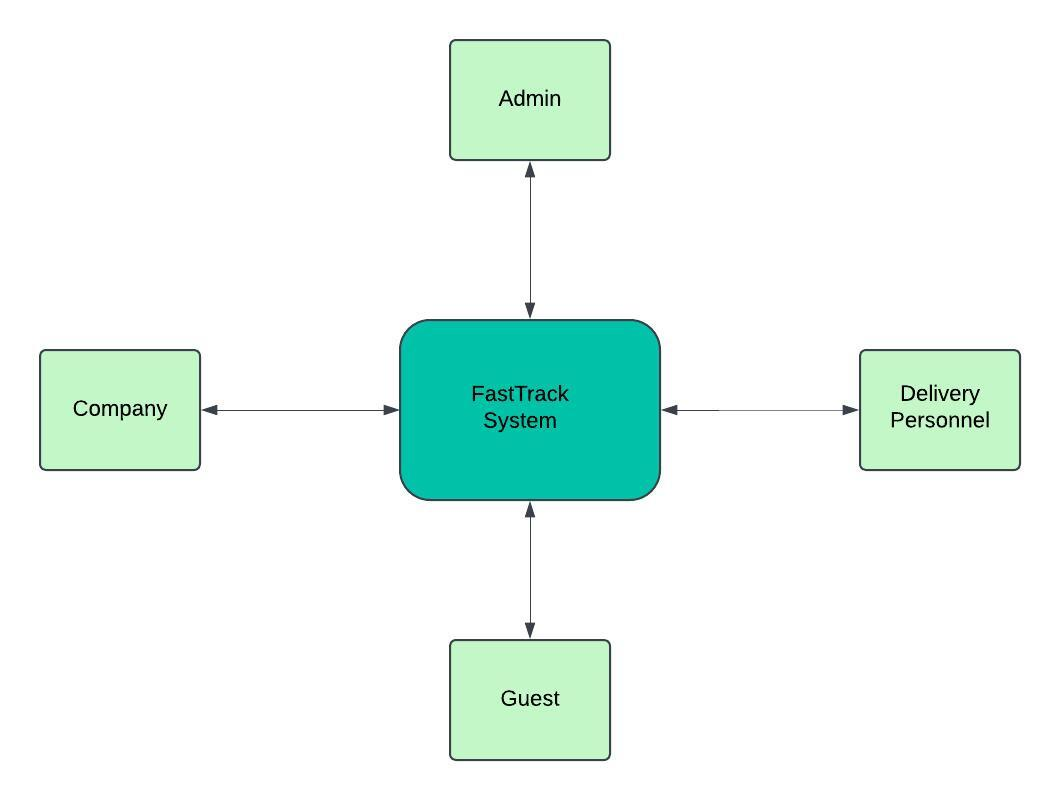
\includegraphics[scale=0.7]{Level 0 Data Flow.jpeg}
    \caption{Level 0 Data Flow}
    \label{fig:level0_data_flow}  % Fix label format (avoid spaces)
\end{figure}
\newpage
\subsubsection{Level 1 Data Flow}
The Level 1 Data Flow Diagram provides a detailed breakdown of the FastTrack System's interactions. It illustrates how different entities (Admin, Company, Delivery Personnel) provide data inputs like registration, package details, and updates, which are processed and stored in the system. The system interacts with data stores for Company Information, Delivery Personnel Data, and Package Details while ensuring smooth validation, updates, and retrieval of necessary information.
\begin{figure}[H]  % Use [H] to keep it under the correct title
\centering
    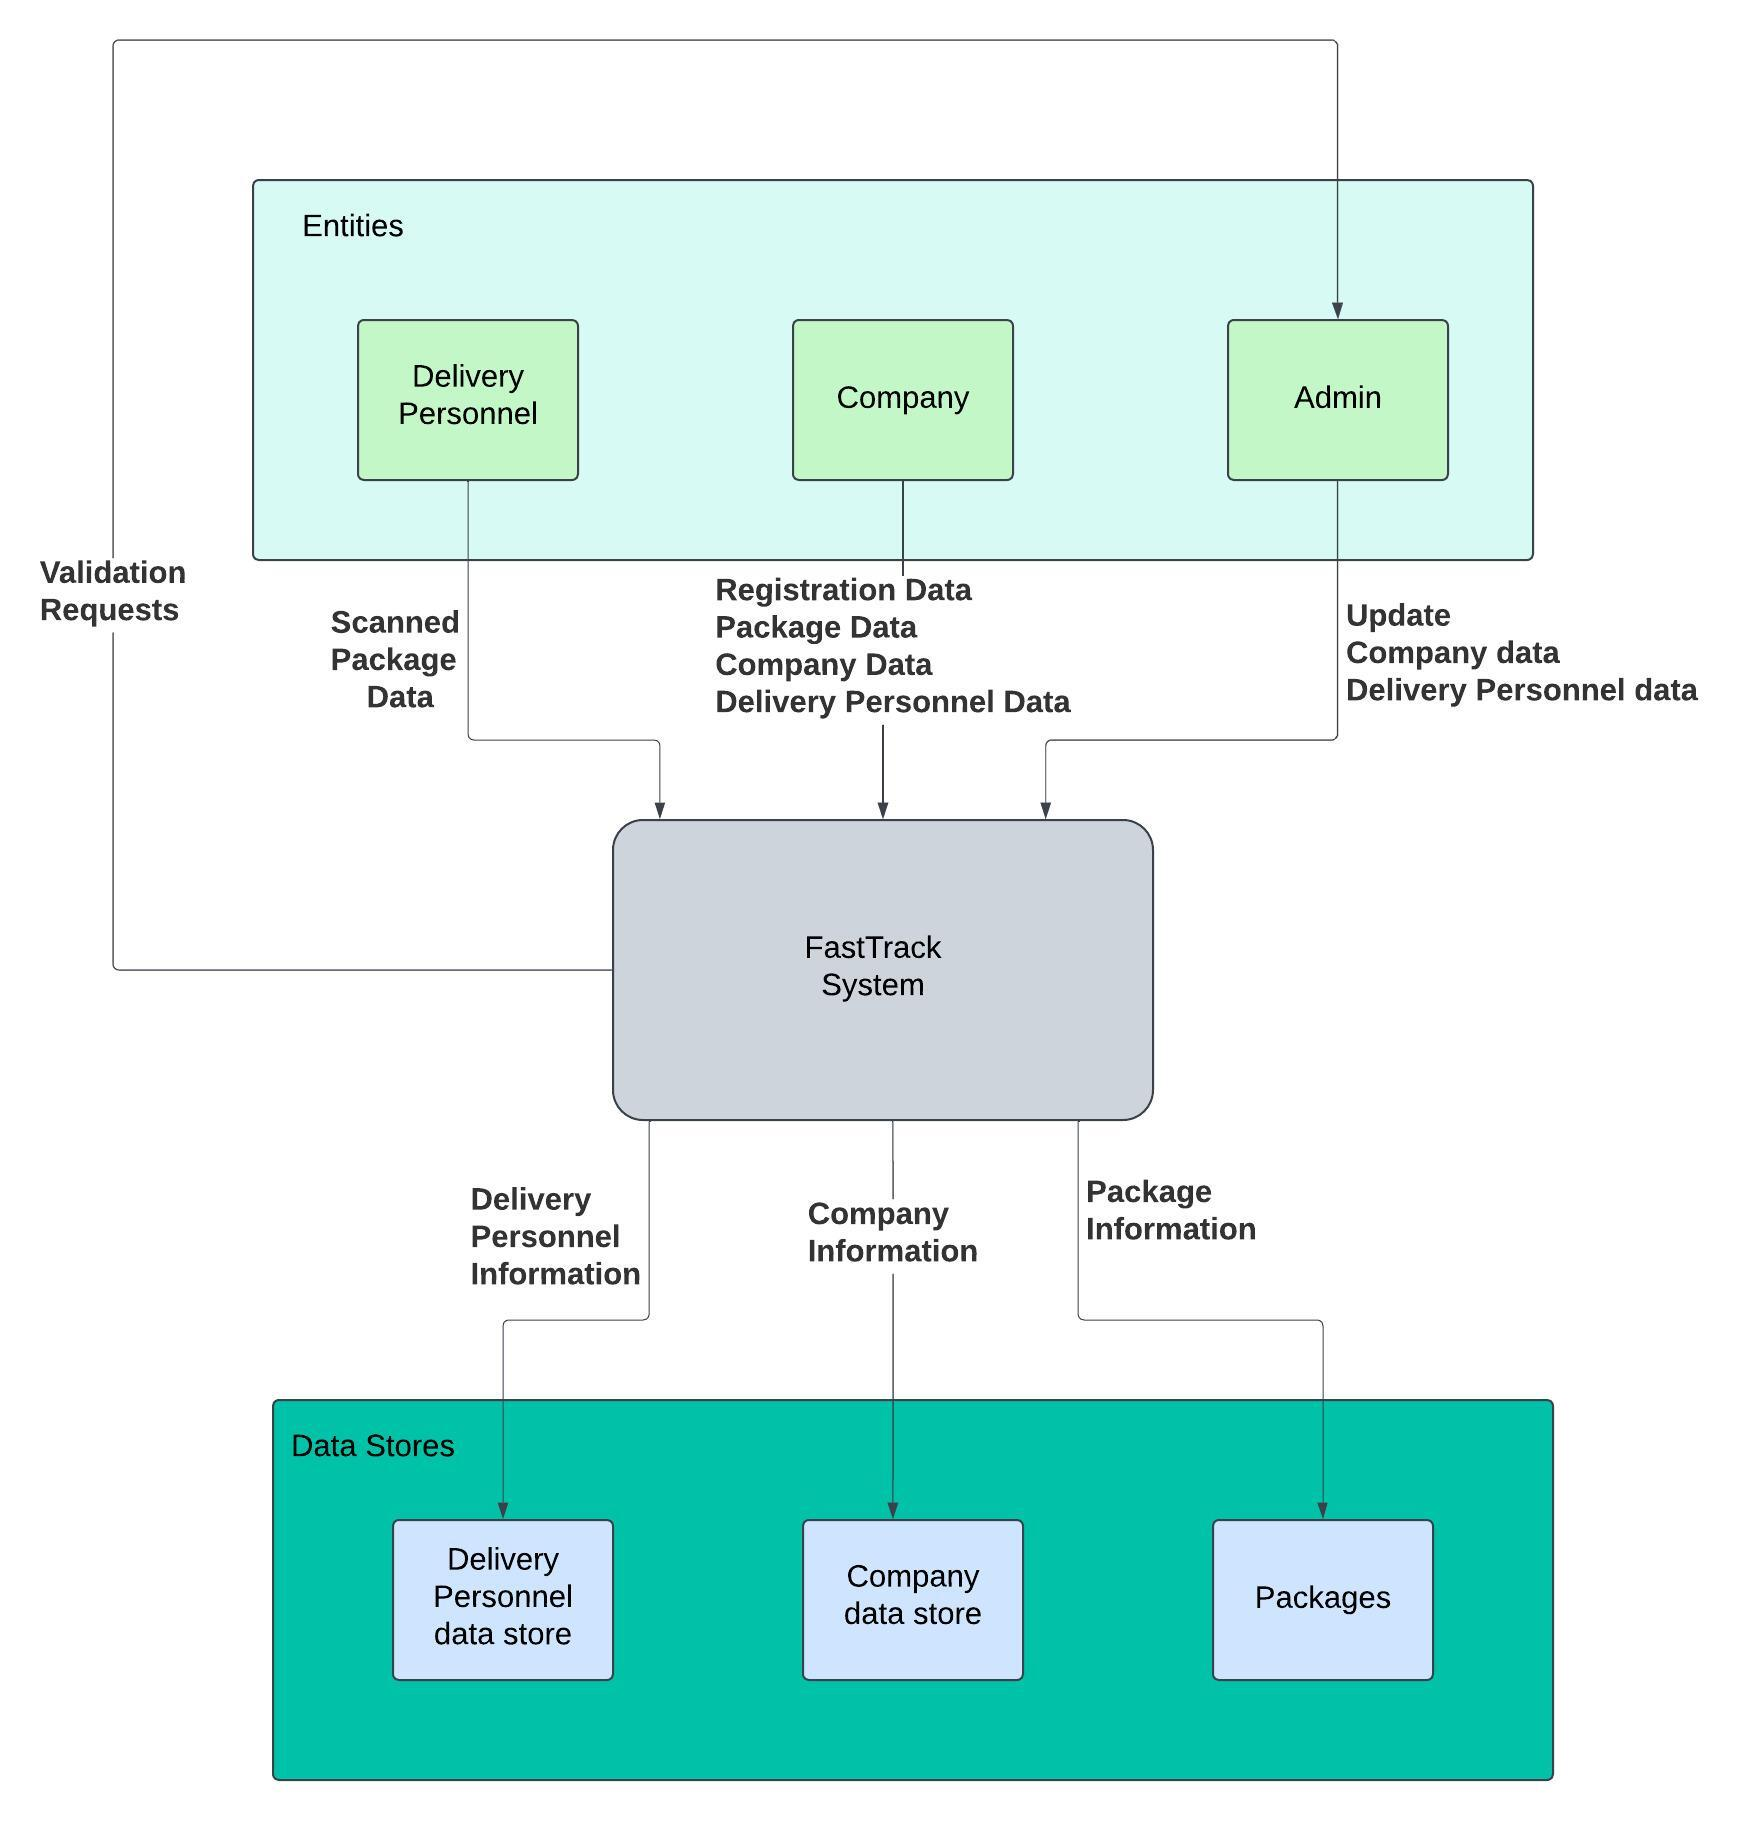
\includegraphics[scale=0.5]{Level 1 Data Flow.jpeg}
    \caption{Level 1 Data Flow}
    \label{fig:level1_data_flow}  % Fix label format (avoid spaces)
\end{figure}
\newpage
\subsection{Use Case Diagram}
The Use Case Diagram for the FastTrack illustrates how different users interact with the system’s functionalities. The main actors are Company, Delivery Personnel, Admin and Guest.
Company can register, arrange packages and generate optimized routes. Delivery Personnel can log in, scan packages, view package details and check optimized routes. Admin is responsible for validating registrations, granting login credentials and updating system information. Guests have limited access, such as browsing the map without logging in.
% \textbf{Actors \& Their Use Cases}
% \begin{enumerate}
%     \item Delivery Personnel 
%     \begin{itemize}
%         \item Login - Logs in using their credentials to manage the system.
%         \item Scan Package - Scans the package details before delivery.
%         \item Package Info - Views package details such as weight, size, and location.
%         \item Optimized Route Info - Gets the best route for deliveries.
%     \end{itemize}
%     \item Company
%     \begin{itemize}
%         \item Register - Registers itself on the platform.
%         \item Login - Logs in using their credentials to manage the system.
%         \item Arrange Packages - Organizes and assigns packages to delivery personnel.
%         \item Generate Optimized Route - Computes the best delivery route for efficiency.
%     \end{itemize}
%     \item Admin
%     \begin{itemize}
%         \item Login - Logs in using their credentials to manage the system.
%         \item Validate Registration - Approves new company registrations.
%         \item Grant Login ID - Provides login credentials to verified companies and personnel.
%         \item Update Info - Updates company and personnel information in the system.
%     \end{itemize}
%     \item Guest
%     \begin{itemize}
%         \item Browse Map - Views the map without logging in.
%     \end{itemize}
% \end{enumerate}

\begin{figure}[H]  % Use [H] to force the position
\centering
    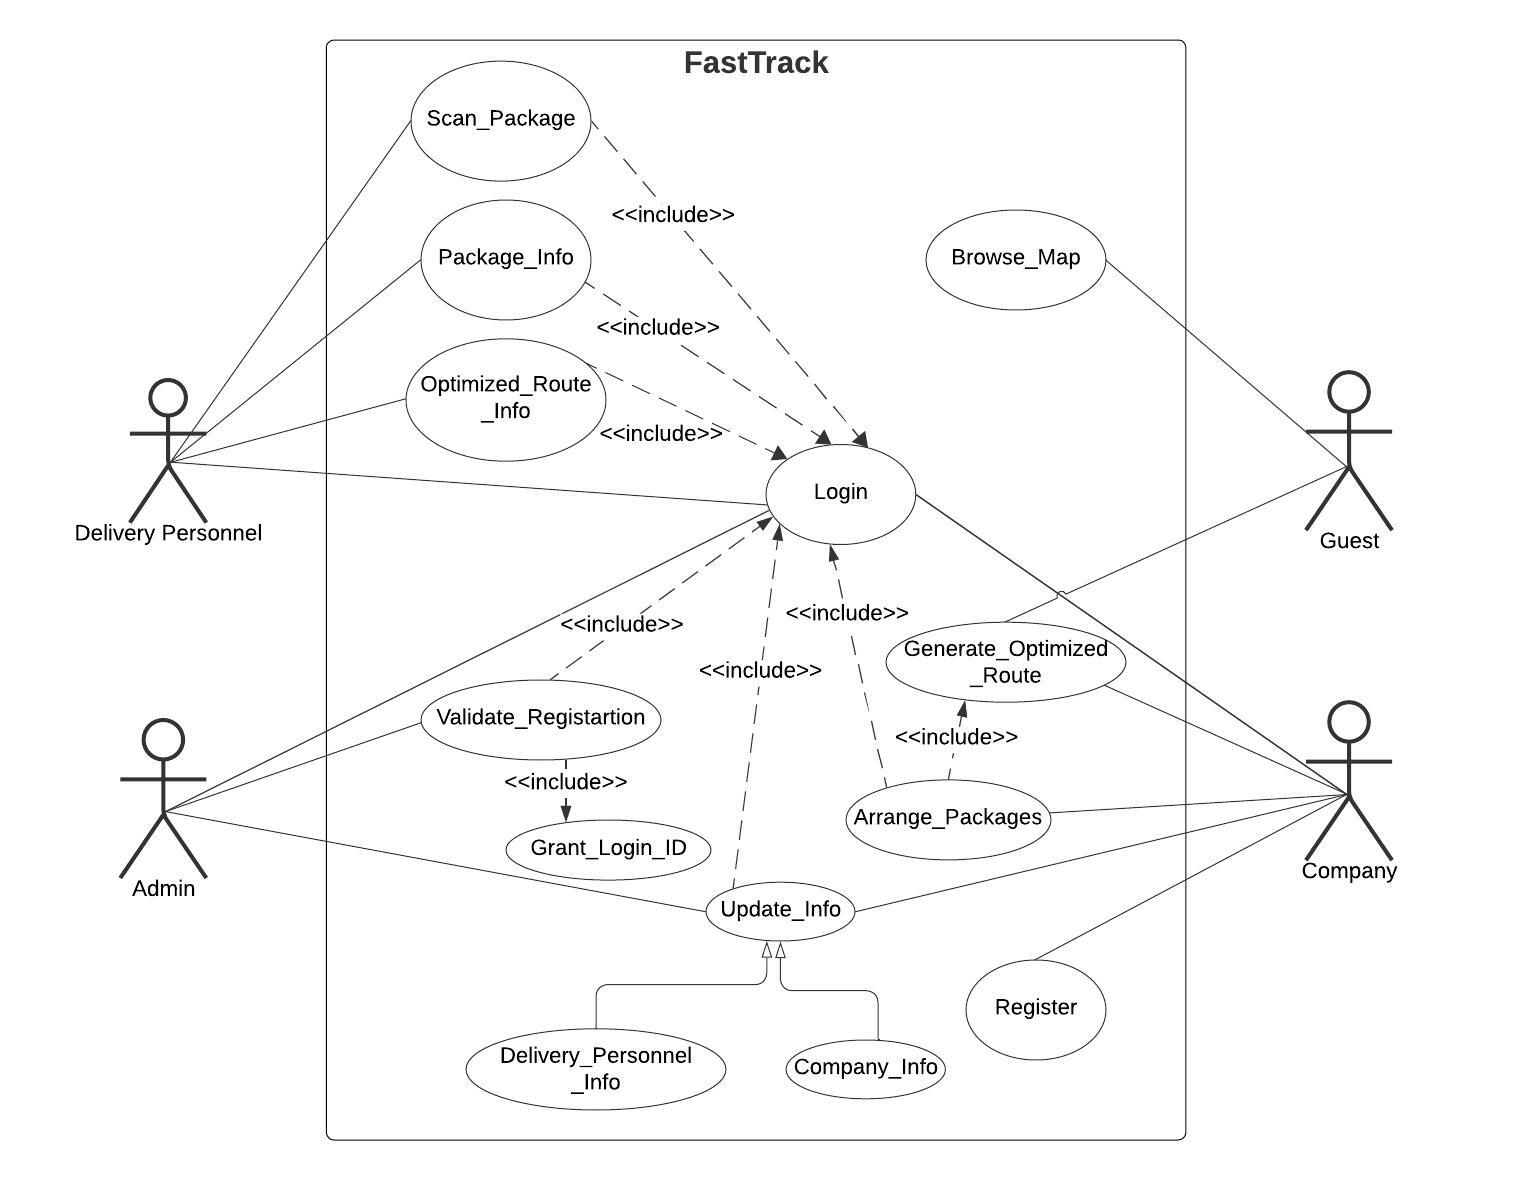
\includegraphics[scale=0.6]{Use case diagram (3).jpeg}
    \caption{Use Case Diagram}
    \label{fig:use_case}
\end{figure}
\newpage
\subsection{System Architecture Diagram}
The System Architecture of Fasttrack consists of a website, a Flutter mobile app, a Firebase database and integration with Google Maps API. The website allows companies to upload package details and assign delivery personnel, while the Flutter app enables delivery personnel to scan packages, receive optimized routes and update their delivery status in real time. Firebase acts as the central database, syncing data between the website and the app. The system also leverages Google Maps API for route optimization and navigation, ensuring efficient deliveries.
\begin{figure}[H]  % Use [H] to force the position
\centering
    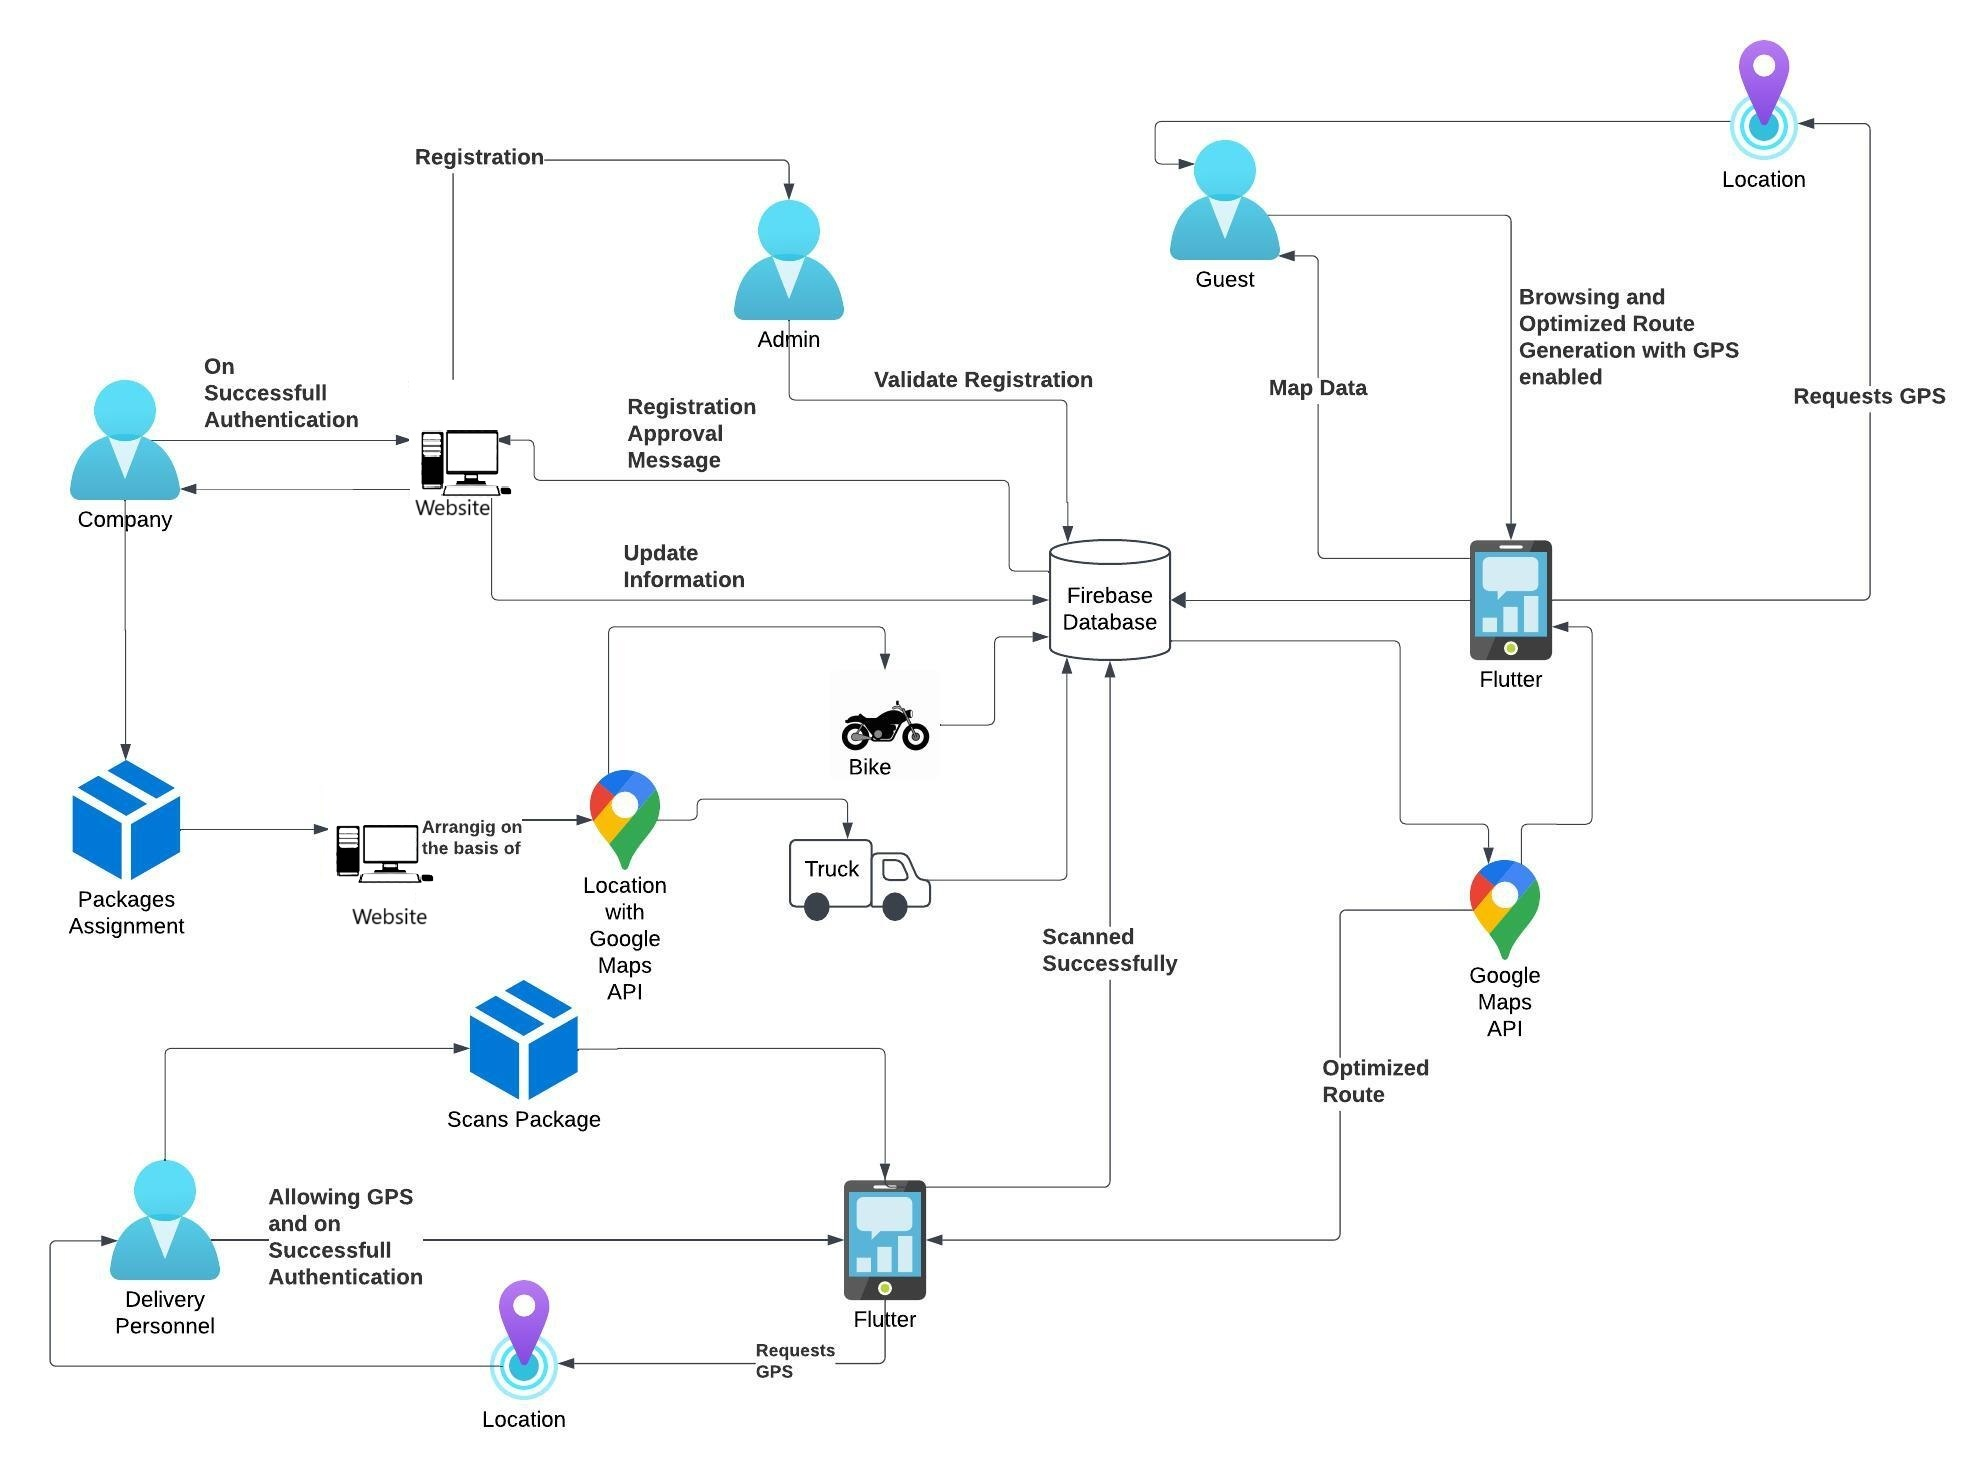
\includegraphics[scale=0.5]{System Architecture.jpeg}
    \caption{System Architecture Diagram}
    \label{fig:system_architecture}
\end{figure}
\newpage
\subsection{Entity-Relationship (ER) Diagram}
The ER Diagram for the FastTrack represents the database structure, showing entities, their attributes and relationships. The main entities are Company, Delivery Personnel, Admin and Package. Company registers on the platform and manages delivery personnel. Delivery Personnel are assigned packages and follow optimized routes for delivery.
Admin verifies company registrations and grants login credentials. Package is linked to a company and assigned to delivery personnel for delivery.
\begin{figure}[H]  % Use [H] to force the position
\centering
    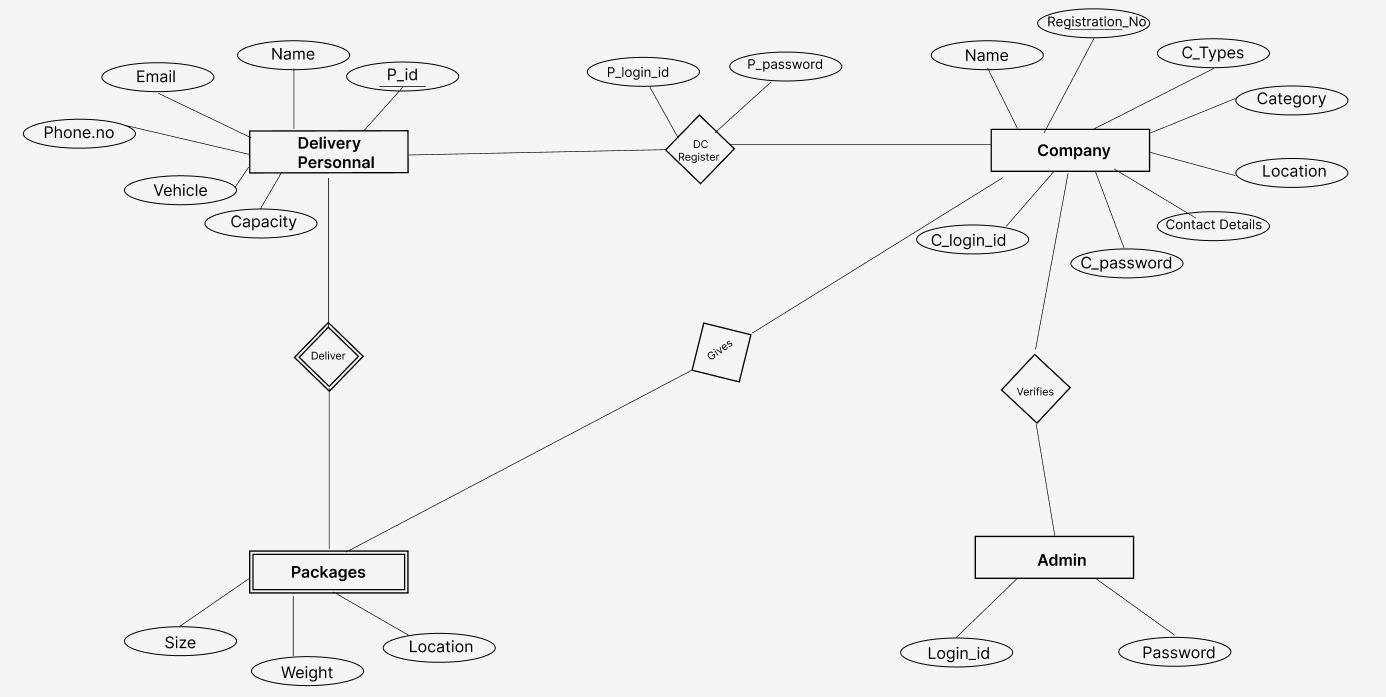
\includegraphics[scale=0.3]{ERdiagram2.jpg}
    \caption{ER Diagram}
    \label{fig:er_diagram2}
\end{figure}
\subsection{Algorithm Modules}
FastTrack incorporates the following algorithm modules:
\begin{itemize}
    \item Authentication Algorithm
    \item Company Registration Algorithm
    \item Update Information Algorithm
    \item Validate Registration Algorithm
        \item Package Assignment Algorithm
    \item Scan Package Algorithm
    \item Retrieve Optimized Route After Scanning Packages Algorithm
    \item Route Optimization with Google Maps API Algorithm
\end{itemize}
\newpage
\section{Detailed Design}
\subsection{Authentication Algorithm}
\SetKwComment{Comment}{/* }{ */}

\begin{algorithm}[hbt!]
\caption{Delivery Personnel or Company or Admin Authentication Algorithm}
\SetKwInOut{Input}{Input}
\SetKwInOut{Output}{Output}
\Input{\textnormal{LoginID and Password}}
\Output{\textnormal{Authentication status (Success/Failure message with token if successful)}}
\textnormal{Input the LoginID and Password from the user.}\\
\textnormal{Search for the LoginID in the user database.}\\
\If{the user with the LoginID is found}{
Validate the Password.\\
\If{the Password matches}{
Generate an Authentication Token.\\
Grant access.\\
Display "Authentication Successful".\\
}
\Else{
Display "Invalid Password,Try Again!".
}
}
\Else{
Display "User Not Found". 
}
\end{algorithm}
\subsection{Company Registration}
\begin{algorithm}[H]
\caption{Company Registration Algorithm}
\SetKwInOut{Input}{Input}
\SetKwInOut{Output}{Output}
\Input{Company Name, Registration Number, Type of Company, Business Category, Address, Contact Details, and Verification Documents}
\Output{Application Number and Validation Status}


Input Company Name, Registration Number, Type of Company, Business Category, Address and Contact Details.\\
Check if the registration number matches the official format using a regular expression.\\
\If{valid}{
    Check if contact details are valid.\\
    \If{valid}{
    Input Certificate of Incorporation, PAN Card and Proof of Address Documents.\\
    \If{Documents uploaded is NULL}{
    Display "Please upload the required documents".
    }
    \Else{
    Generate an application tracking number.\\
    Display "Validation Status: Pending Approval".
    }
    }
    \Else{Display "Invalid Contact Details".}
}
\Else{Display "Invalid Registration Number".}
\end{algorithm}
\subsection{Update Information Algorithm}
\begin{algorithm}[H]
\caption{Update Information}
\SetKwInOut{Input}{Input}
\SetKwInOut{Output}{Output}
\Input{
\textnormal{User Role: Admin, Company or Delivery Personnel \\Update options: Address, Contact Information, Business Category}
}
\Output{ 
    \textnormal{Update Status (Success or Failure)}\\
}
Input User Role: Admin, Company or Delivery Personnel.
\\
Verify User Login using Algorithm 1.\\
Capture the fields the user wants to update.\\
Access the corresponding database table.\\
Update the relevant fields with the new details.\\
\If{the database update fails}
{
Display "Error updating information. Please try again later".\\
Set Update Status as "Failure".\\
\Else{
Display "Information updated successfully".\\
Set Update Status as "Success".}
}
\end{algorithm}
\subsection{Validate Registration Algorithm}
\begin{algorithm}
\caption{Validate Registration}
\SetKwInOut{Input}{Input}
\SetKwInOut{Output}{Output}
\Input{
\textnormal{Certificate of Incooperation, PAN Number and Proof of Address}
}
\Output{Validation status (Valid/Invalid)
}

Input Certificate of Incooperation, PAN Number and Proof of Address.\\
Ensure the Certificate of Incorporation is uploaded.\\
Verify that the PAN Card matches the company name format.\\
Check if the Proof of Address is valid.\\
\If{All validation is done}{
set Validation Status as "Valid".\\
sent LoginID and temporary password to the company's email address.\\
\Else{
set Validation Status as "Invalid".\\
sent a message "Validation Failed due to incorrect document submission" to the company's email address.\\
}
}
\end{algorithm}
\subsection{Package Assignment Algorithm}
\small 
\begin{algorithm}
\caption{Package Assignment}
\SetKwInOut{Input}{Input}
\SetKwInOut{Output}{Output}
\Input{
    \textnormal{An Excel sheet, which includes package ID, location, weight, size, and date.}\\
    	\textnormal{Average weight and size capacity of the vehicles used for delivery.}\\
        \textnormal{Warehouse location}
}
\Output{
    \textnormal{Table with assigned Employee ID, Package ID, Location, and Date}
}
Dividing packages into four quadrants based on their delivery location:
Quadrants = {"NE": [], "NW": [], "SW": [], "SE": []}\\

Categorize packages by Algorithm 6\\

Categorize packages by vehicles based on, bikes can carry packages labeled lvs, ls, lm, ms, and mm, while trucks can carry packages labeled ll, ml, hs, hm, hl, hym, and hyl.\\

Calculate the total weight and size for both bikes and trucks, add any remaining weight and size to the current weighted size during the calculation.\\

Use Algorithm 7 to find number of employees for bike and truck.\\

Input Number of Employees for bikes and trucks\\

Assign packages to bike employees by Algorithm 8\\

\If{Total weight of Bpackage_remaining $\geq $125kg
}{Average weight of truck = 125kg\\
Average size of truck = 500cm³\\
\[
m = \frac{\text{Total weight of Bpackage remaining}}{\text{Average weight of truck}}
\]

\[
n = \frac{\text{Total size of Bpackage remaining}}{\text{Average size of truck}}
\]

\[
\text{Truck\_employee2} = \max(m, n)
\]

\[
\text{Total\_Truck\_employee} = \text{Truck\_employee} + \text{Truck\_employee2}
\]}

Assign packages to truck employees by Algorithm 9\\
\end{algorithm}

\begin{algorithm}
\caption{Categorize Packages}
\SetKwInOut{Input}{Input}
\SetKwInOut{Output}{Output}
\Input{
\textnormal{package ID, location, weight and size}
}
\Output{ 
    \textnormal{Categorized package list 
}
}
\ForEach{weight in packages}{
Extract weight $w$ and size $s$ from $p$\;
 \If{$w < 2$ \textbf{and} $s <$ verysmall}{
        Assign $p$ to category \texttt{lvs}\;
    }
    \ElseIf{$w < 2$ \textbf{and} $s <$ small}{
        Assign $p$ to category \texttt{ls}\;
    }
    \ElseIf{$w < 2$ \textbf{and} $s <$ medium}{
        Assign $p$ to category \texttt{lm}\;
    }
    \ElseIf{$2 < w < 5$ \textbf{and} $s <$ small}{
        Assign $p$ to category \texttt{ms}\;
    }
    \ElseIf{$2 < w < 5$ \textbf{and} $s <$ medium}{
        Assign $p$ to category \texttt{mm}\;
    }
    \ElseIf{$w < 2$ \textbf{and} $s <$ large}{
        Assign $p$ to category \texttt{ll}\;
    }
    \ElseIf{$2 < w < 5$ \textbf{and} $s <$ large}{
        Assign $p$ to category \texttt{ml}\;
    }
    \ElseIf{$5 < w < 15$ \textbf{and} $s <$ small}{
        Assign $p$ to category \texttt{hs}\;
    }
    \ElseIf{$5 < w < 15$ \textbf{and} $s <$ medium}{
        Assign $p$ to category \texttt{hm}\;
    }
    \ElseIf{$5 < w < 15$ \textbf{and} $s <$ large}{
        Assign $p$ to category \texttt{hl}\;
    }
    \ElseIf{$w > 15$ \textbf{and} $s <$ medium}{
        Assign $p$ to category \texttt{hym}\;
    }
    \ElseIf{$w > 15$ \textbf{and} $s <$ large}{
        Assign $p$ to category \texttt{hyl}\;
    }
}
\end{algorithm}

\begin{algorithm}
\caption{Assigning Algorithm for Bike and Truck Employees}
\SetKwInOut{Input}{Input}
\SetKwInOut{Output}{Output}
\Input{
    \textnormal{Packages with weight, size, and location.}\\
    \textnormal{Vehicle capacity (average weight and size).}
}
\Output{
    \textnormal{Assigned employees and optimized routes.}
}

\While{Total\_Weight\_Vehicle $\neq$ 0}{ 
    
    \While{\textnormal{Quadrants changing}}{
        
        \While{\textnormal{Each employee is processing}}{ 
            
            \While{Average\_Weight $\neq$ 0 \textbf{and} Average\_Size $\neq$ 0}{
                Assign package\;
                Update Average\_Weight, Average\_Size\;
                
                \If{\textnormal{Remaining space but no suitable package}}{
                    
                    \If{Average\_Weight $>$ 4}{
                        Move to next quadrant (i → i+1)\;
                        Assign available package\;
                    }
                    
                    \If{Average\_Weight $<$ 4}{
                        Move to next quadrant (i → i+1)\;
                        \If{Average\_Weight == Package\_Weight \textbf{and} Average\_Size == Package\_Size}{
                            Perform route optimization\;
                            Compute shortest path (Dijkstra’s algorithm)\;
                            \If{Distance $<$ MAX\_DISTANCE}{
                                Assign package and update weight/size\;
                            }
                        }
                    }
                }
            }
        }
    }
}
\end{algorithm}
\begin{algorithm}
\caption{Assigning Packages to Bike Employees}
\SetKwInOut{Input}{Input}
\SetKwInOut{Output}{Output}
\Input{
    \textnormal{Bike employees count, available employees, and assigned packages.}
}
\Output{
    \textnormal{Updated package assignment and remaining packages.}
}

\If{Bike\_employees == Available\_employeesB}{
    Assign packages using \texttt{assigned\_packages[]} from Algorithm 7\;
}

\If{Bike\_employees > Available\_employeesB}{
    Assign packages to available employees\;
    Store remaining packages in \texttt{Bpackages\_remaining}\;
    Prioritize remaining packages for the next working day\;
}

Calculate total weight and size of \texttt{Bpackage\_remaining}\;

\end{algorithm}
\begin{algorithm}
\caption{Truck Employee Allocation and Package Assignment}
\SetKwInOut{Input}{Input}
\SetKwInOut{Output}{Output}
\Input{
    \textnormal{Total Truck Employees required (\texttt{Total\_Truck\_employees})}\\
    \textnormal{Available Truck Employees (\texttt{Available\_EmployeesT})}
}
\Output{
    \textnormal{Assigned employees and remaining packages}
}

\If{Truck\_employees == Available\_EmployeesT}{
    Assign packages to employees\;
    \texttt{Bpackage\_remaining} remains unchanged and is prioritized for the next working day\;
}

\If{Truck\_employees > Available\_EmployeesT}{
    Assign packages to \texttt{Available\_EmployeesT}\;
    Store remaining packages in \texttt{Tpackage\_remaining} and prioritize for the next working day\;
    \texttt{Bpackage\_remaining} remains unchanged and prioritized for the next working day\;
}

\If{Total\_Truck\_employees == Available\_EmployeesT}{
    \If{Truck\_employees == Available\_EmployeesT - Truck\_employee2}{
        Assign packages to employees\;
        Assign \texttt{Bpackage\_remaining} to employees\;
    }
}

\If{Total\_Truck\_employees > Available\_EmployeesT \textbf{and} Truck\_employees < Available\_EmployeesT}{
    \texttt{Emp} $\gets$ Available\_EmployeesT - Truck\_employees\;
    
    \If{Truck\_employees == Available\_EmployeesT - Emp}{
        Assign packages to employees\;
    }

    \If{Truck\_employee2 > Emp}{
        Assign \texttt{Bpackage\_remaining} to \texttt{Emp}\;
        Store remaining packages in \texttt{Bpackages\_remaining} and prioritize for the next working day\;
    }
}

\end{algorithm}
\subsection{Scan Package}
\begin{algorithm}[H]
\caption{Scan Package}
\SetKwInOut{Input}{Input}
\SetKwInOut{Output}{Output}
\Input{
\textnormal{Package ID (from the scanned QR code)}
}
\Output{ 
    \textnormal{Scanning Status (Success or Failure) 
}
}
Verify Login using Algorithm 1.\\
Extract the Package ID from the scanned data.\\
Check if the Package ID exists in the system's database.\\
\If{not found}
{
Display "Invalid Package ID. Please scan a valid package".\\
Set Scanning Status as "Failure".\\
}
\Else{
Update the package record in the database\\
Set Scanning Status as "Success."\\
Display "Package successfully scanned and assigned for delivery."\\
}
\end{algorithm}
\subsection{Retrieve efficient Route After Scanning Packages}
\begin{algorithm}[H]
\caption{Retrieve efficient Route After Scanning Packages Algorithm}
\SetKwInOut{Input}{Input}
\SetKwInOut{Output}{Output}
\Input{
\textnormal{Delivery Personnel ID\\
Scanned Package IDs}
}
\Output{ 
    \textnormal{
    Route Map (Efficient delivery route) or Error Message
}\\
}
Verify Login using Algorithm 1.\\
Ensure all assigned Package IDs are scanned.\\
\If{not all assigned packages are scanned}
{Display "Not all assigned packages are scanned."}
\Else{
Retrieve the efficient Route generated by the company for this specific set of packages.\\
\If{no route exists}
{Display "Optimized route not available."}

\Else{
Display the efficient Route Map on the delivery personnel’s interface.
}}
\end{algorithm}
\newpage
\subsection{Route Optimization with Google Maps API Algorithm}
\begin{algorithm}
\caption{Route Optimization with Google Maps API}
\SetKwInOut{Input}{Input}
\SetKwInOut{Output}{Output}
\Input{
\textnormal{Delivery locations (latitude, longitude)}
}
\Output{ 
    \textnormal{Optimized delivery route and total distance}\\
}
Input Delivery Locations as latitude and longitude pairs.\\
Send the locations to Google Maps Distance Matrix API.\\
Receive pairwise distances and travel times between all locations.\\
Set the first location as the starting point.\\
Initialize an empty route list and add the starting location.\\
Optimize Route Using Greedy Algorithm.\\
\While{there are unvisited locations}
{
    Find the nearest unvisited location using the distance matrix\\
    Add the nearest location to $route$\\
    Mark the location as visited\\
}
Add the starting location to the end of the route to complete the cycle.\\
For calculating the total distance, sum the distances between consecutive locations in the route using the distance matrix.\\
Display the optimized route sequence and integrate with Google Maps for visualization.\\
Print the total distance.\\
\end{algorithm}
\section{Summary}
Chapter 3 of the software development life cycle (SDLC) delves into the design phase, transitioning
from problem identification to solution planning. It encompasses two key stages: System Design and
Detailed Design. The System Design phase defines key system components, interactions and data
flow using DFDs, use case diagrams, system architecture and ER diagrams. The Detailed Design
phase elaborates on essential algorithms, including authentication, company registration, update
information, validate registration, package assignment, scan package, retrieving efficient route and
route optimization.
\chapter{Implementation}
\label{Implementation}

% Software & Hardware Requirements
% Code implementation details (brief descriptions, screenshots)
% Features and functionalities

\section{Software Requirements}
\subsection{Operating System Requirements}
Fasttrack requires a modern operating system that supports web browsers and mobile applications. The web platform runs on Windows 7 and above while the mobile app is compatible with Android 7.0 and above. A 64-bit processor with at least 4GB RAM is recommended for smooth performance. The system should support Google Chrome, Firefox, Edge, or Safari for optimal web functionality. 
\subsection{Tools Used}
Various tools that are utilized for the implementation of Fasttrack are:
\subsubsection{HTML}
The FastTrack website uses HTML to structure its content, including login, package management and employee assignment sections. It employs semantic elements like <form>, <table>, <div>, and <button> to enhance accessibility and organization. The login and registration forms use <input> fields for credentials, while <table> elements display package and employee details. Navigation is handled with <nav>, and <header> and <footer> provide structured branding. HTML ensures compatibility across devices and browsers, improving SEO and accessibility. Combined with CSS and JavaScript, it enables dynamic interactions like employee assignment. HTML also integrates seamlessly with Firebase and Flask for backend operations.
\subsubsection{CSS}
The FastTrack web application uses CSS to enhance the visual appeal and responsiveness of its interface. It employs Flexbox and Grid for layout management, ensuring a structured and adaptable design. Custom styling is applied to buttons, tables and forms for a professional look and improved usability. Media queries make the website responsive across different screen sizes, from desktops to mobile devices. Hover effects and animations improve user interaction, making navigation more intuitive. CSS variables and reusable classes ensure consistency across pages. The design follows a clean and modern aesthetic, improving the user experience for companies and employees.
\subsubsection{JavaScript}
The FastTrack website uses JavaScript to add interactivity and dynamic functionality. It handles form validation, ensuring correct user input before submission. AJAX requests enable seamless data fetching from the backend without reloading the page. Event listeners manage user interactions, such as button clicks and form submissions. JavaScript updates the UI dynamically, like displaying assigned packages without refreshing. It integrates with Firebase for real-time updates on package assignments and employee status. Third-party libraries, such as Google Maps API, enhance location-based features. The script ensures a smooth and efficient user experience across the platform.
\subsubsection{Python}
The FastTrack website uses Python for backend development, primarily with Flask. Flask handles HTTP requests and serves data to the frontend via REST APIs. It integrates with Firebase Firestore, managing company, employee and package data efficiently. Python processes uploaded Excel files, extracting package details for assignment. The employee assignment algorithm is implemented in Python, optimizing route efficiency. It also manages authentication and authorization, ensuring secure access to company and admin functionalities. Python’s flexibility and Flask’s lightweight nature enable a scalable and efficient backend for FastTrack.
\subsubsection{Flutter}
The FastTrack mobile app is built using Flutter, a cross-platform framework for developing high-performance applications. Dart is the primary language, enabling smooth UI and efficient state management. The app integrates with Firebase Authentication for secure employee login and Firestore for real-time package updates. Google Maps API is used for location input, navigation, and route optimization, ensuring efficient deliveries. The app supports push notifications via Firebase to keep employees updated. With Flutter's widget-based approach, the app offers a responsive and interactive user experience across Android devices.
\subsubsection{Firebase}
Firebase is essential for the FastTrack system, providing a secure and scalable backend. Firebase Authentication ensures safe logins for companies and employees. Cloud Firestore stores real-time data, including employee details, package assignments and delivery status updates. Firebase Hosting can be used to deploy the web portal efficiently. With Google’s robust infrastructure, Firebase enables seamless data synchronization and real-time updates across devices. It simplifies backend management, eliminating the need for a separate server while ensuring high availability and security.
\subsubsection{Google Maps API}
The Google Maps API is used in the FastTrack to enhance location-based features in the Flutter app. It enables map rendering, real-time GPS tracking, and dynamic routing for delivery personnel. Directions API helps in generating optimized routes for multiple deliveries, ensuring efficient navigation. Geocoding API converts addresses into coordinates for precise location storage. Maps customization allows branding adjustments to align with FastTrack’s theme. With real-time updates and interactive map controls, the API ensures a seamless and intuitive delivery experience.
\subsubsection{Supabase}
Supabase is used for storing images in FastTrack as a scalable and secure alternative to Firebase Cloud Storage. It provides PostgreSQL-backed storage, ensuring efficient retrieval and management of profile and package images. It provides a direct URL link for each uploaded image, making it easy to retrieve and display images in the FastTrack app. These links can be stored in Firestore alongside other user or package data for quick access. 
\section{Hardware Requirements}
\subsection{Website}
\begin{enumerate}
    \item Processor: At least an Intel i3 (or AMD equivalent), but i5/i7 is recommended for smooth multitasking.
    \item RAM: Minimum 4GB, recommended 8GB or higher for handling multiple browser tabs and development tools.
    \item Internet Connection: A stable broadband connection (at least 10 Mbps) for real-time interactions with cloud-based services.
\end{enumerate}
\subsection{Mobile App}
\begin{enumerate}
    \item Processor: A 1.4 GHz or higher multi-core processor to ensure smooth app execution and real-time processing.
    \item RAM: At least 2GB for basic performance, with 4GB or more recommended for handling maps and real-time updates efficiently.
    \item Connectivity: Stable 4G/5G, GPS and Wi-Fi support for seamless real-time data transmission and location tracking.
\end{enumerate}
\section{Code Implementation Details}
\subsection{Authentication \& Authorization}
FastTrack uses Firebase Authentication for secure login and access control. Employees and companies authenticate using email and password, while the system verifies credentials and maintains session states. The authentication logic ensures that only authorized users can access package details and employee assignments.
\subsection{Package Assignment}
Package details are uploaded via an Excel file, processed using Python (Flask), and stored in Firestore. Each package entry includes recipient details, location coordinates, and assigned delivery personnel. The system updates package status dynamically based on delivery progress.
\subsection{Employee Assignment}
The system calculates the required number of employees based on the uploaded package data. Companies select available employees and packages are automatically assigned using a assignment algorithm that minimizes travel distance. The assignments are updated in Firestore for real-time access by employees.
\subsection{Route Optimization \& Navigation}
The Google Maps API is integrated into the mobile app to assist delivery personnel. Employees can view optimized routes and track package drop-off points.
Optimized route generation in FastTrack is based on a greedy algorithm, ensuring efficient delivery route planning. The app dynamically updates routes when a delivery is completed.
\subsection{Real-time Updates \& Notifications}
Firestore enables real-time synchronization of package assignments and status updates across the system. Employees receive push notifications (Firebase) for new assignments and delivery updates.
\subsection{Screenshots}
\begin{figure}[H]
\centering
\begin{minipage}{0.6\textwidth}
    \centering
    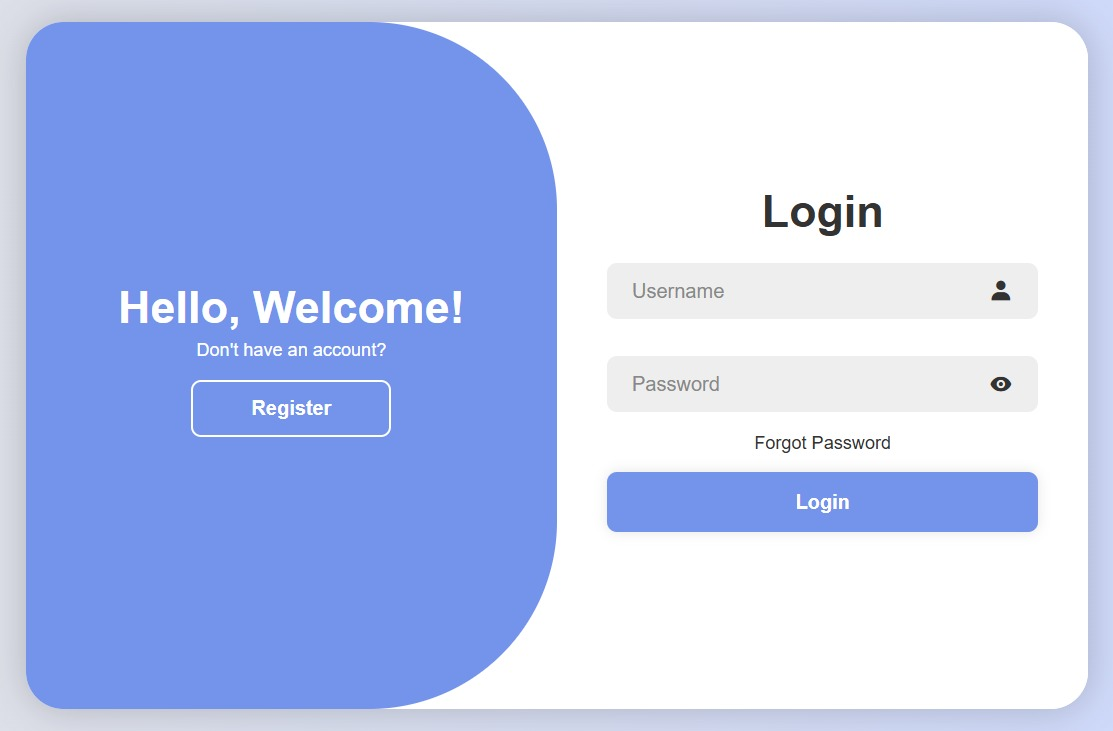
\includegraphics[width=\linewidth]{4/Website_Login.jpg}
    \label{fig:authentication1}
\end{minipage}%
\hspace{5mm}
\begin{minipage}{0.3\textwidth}
    \centering
    \includegraphics[width=\linewidth]{4/Mobile_login.jpg}
    \label{fig:authentication2}
\end{minipage}
\caption{Authentication \& Authorization}
\label{fig:authentication_combined}
\end{figure}
\begin{figure}[H]  % Use [H] to force the position
\centering
    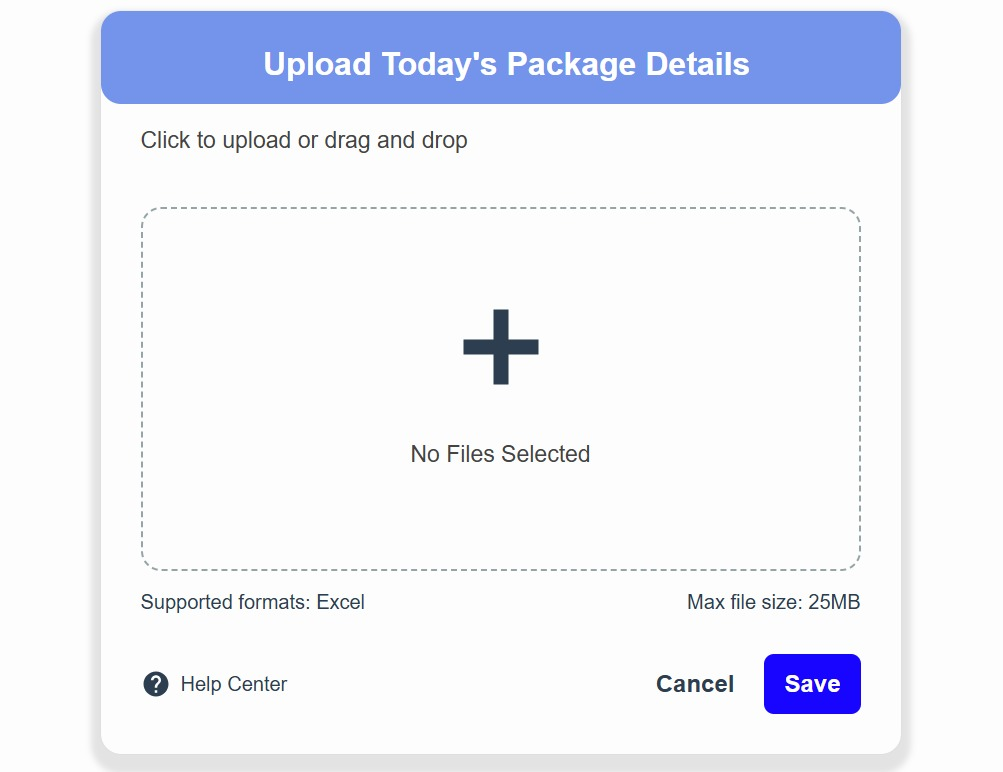
\includegraphics[scale=0.3]{4/Package_Upload.jpg}
    \caption{Package Assignment}
    \label{fig:package_upload}
\end{figure}
\begin{figure}[H]  % Use [H] to force the position
\centering
    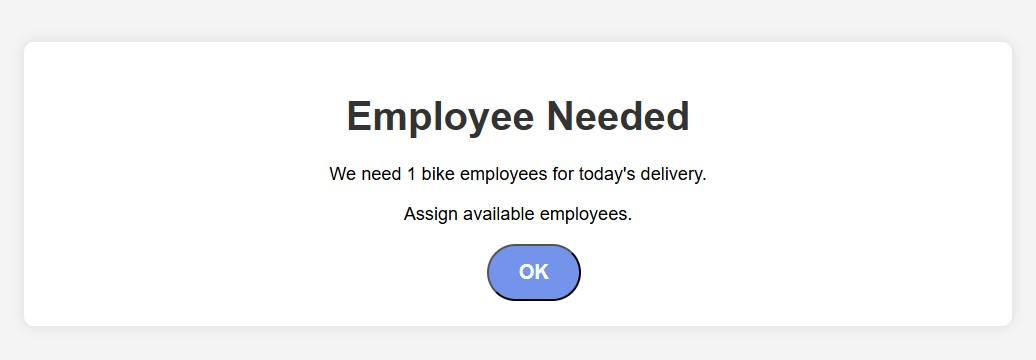
\includegraphics[scale=0.5]{4/Employee1.jpg}
    \caption{Employee Assignment}
    \label{fig:employye_assignment}
\end{figure}
\begin{figure}[H]
\centering
\begin{minipage}{0.24\textwidth}
    \centering
    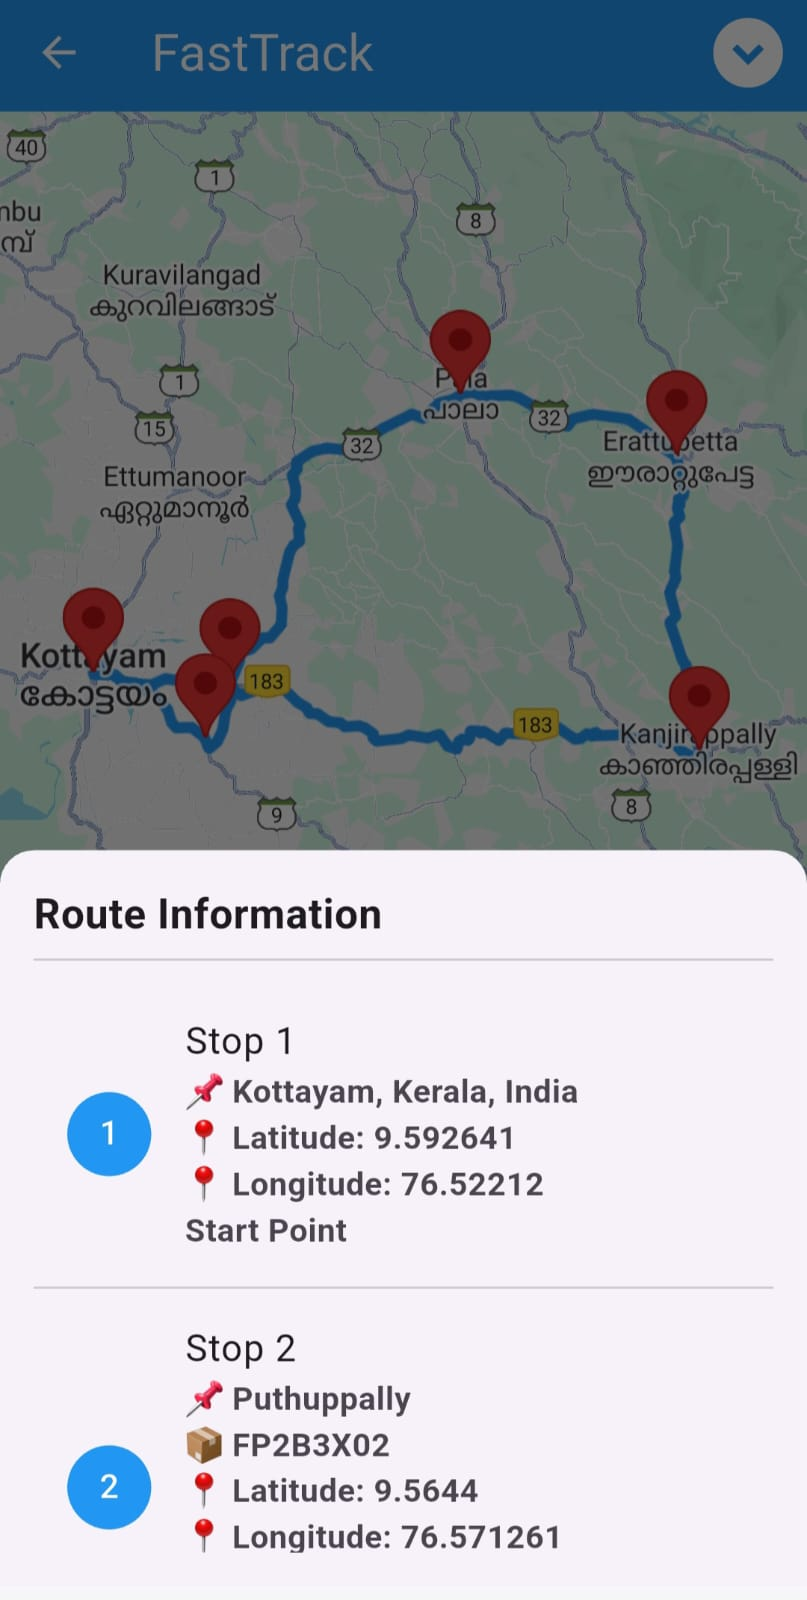
\includegraphics[width=\linewidth]{4/Route_Optimization2.jpg}
    \label{fig:route_optimization2}
\end{minipage}%
\hspace{5mm}
\begin{minipage}{0.24\textwidth}
    \centering
    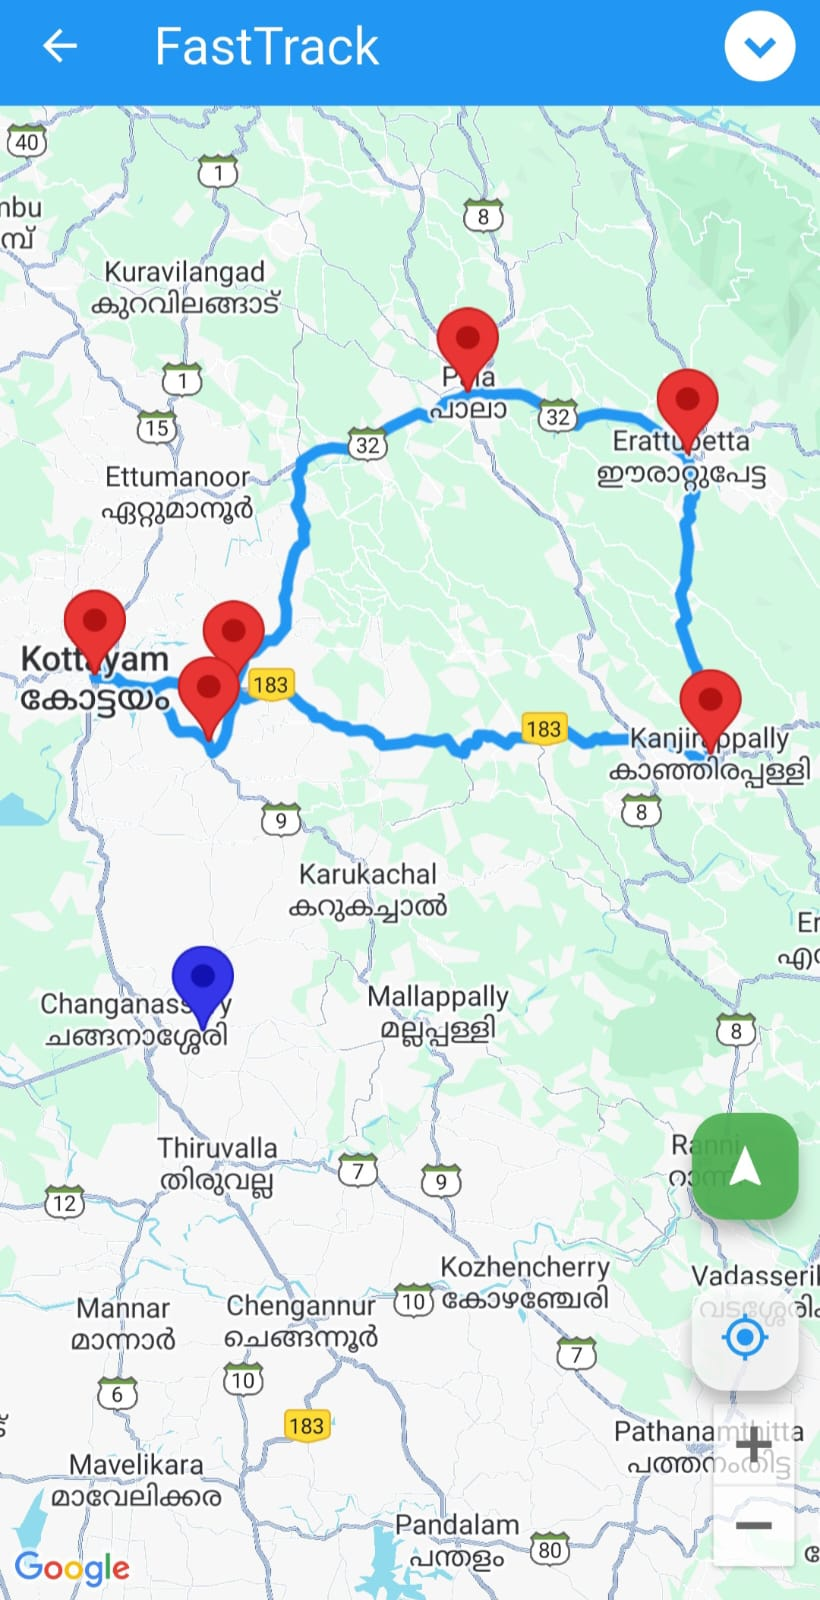
\includegraphics[width=\linewidth]{4/Route_Optimization1.jpg}
    \label{fig:route_optimization1}
\end{minipage}
\caption{Route Optimization and Navigation}
\label{fig:route_optimization_combined}
\end{figure}
\begin{figure}[H]
    \centering
    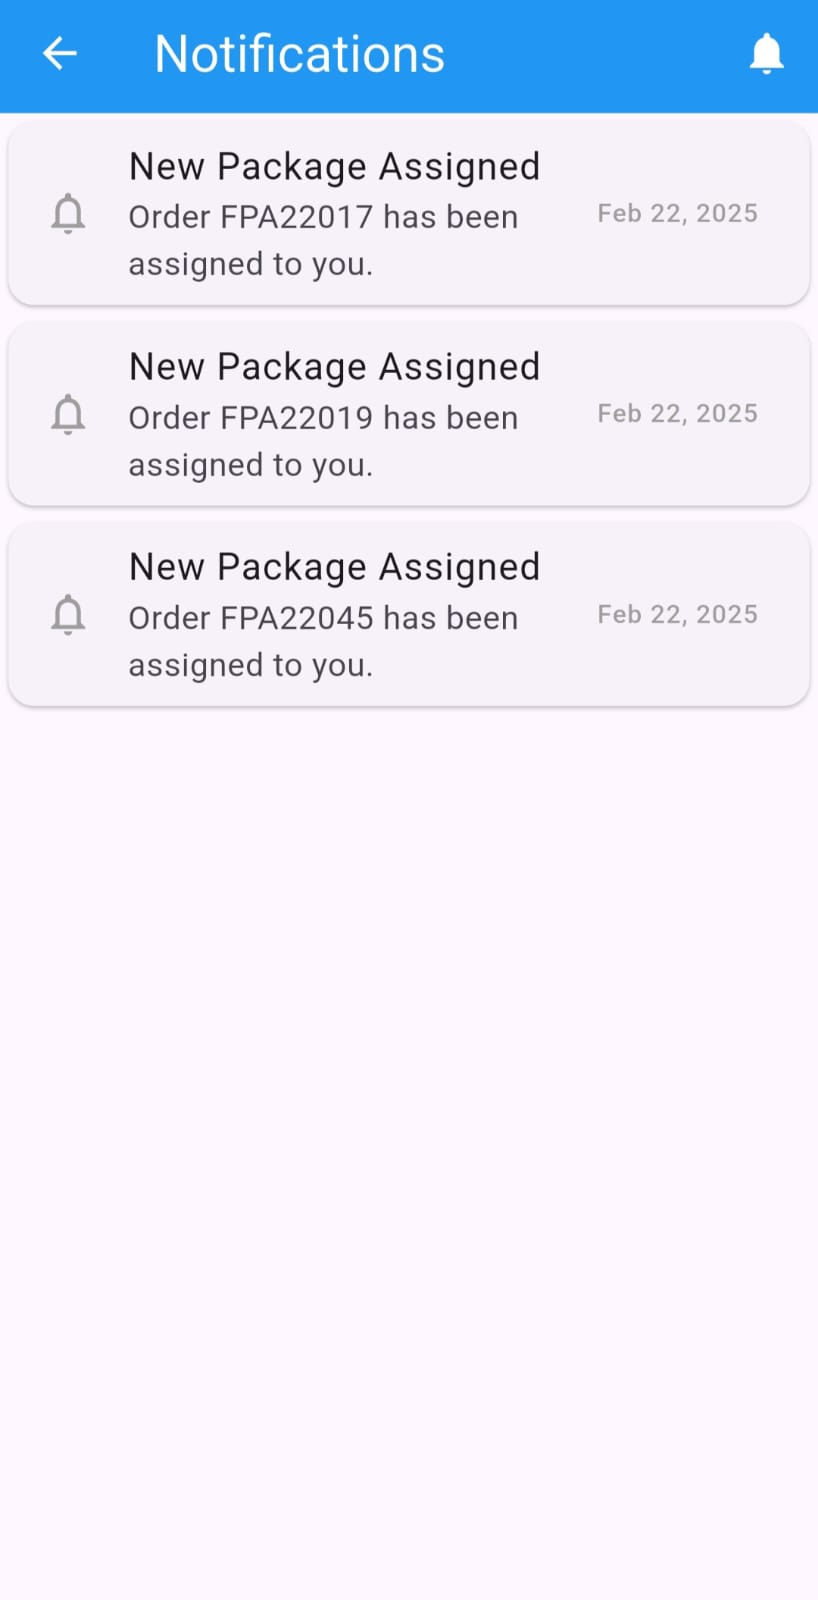
\includegraphics[width=0.24\linewidth]{4/Notification.jpg}
    \caption{Notifications}
    \label{fig:notificationl}
\end{figure}
\newpage
\section{Features and Functionalities}
\subsection{User Authentication \& Management}
\begin{itemize}
    \item Companies can register with required details.
    \item They can login securely using Firebase Authentication.
    \item Companies can add, edit and manage delivery personnel.
    \item Each company gets a unique 5-character alphanumeric ID (FCXXX).
    \item Each employee gets a unique 8-character alphanumeric ID (FDXXXYYY), where XXX wil be Company ID.
    \item Each packet will gets a unique 8-character alphanumeric ID (FPXXXYYY), where XXX wil be Company ID.
\end{itemize}
\subsection{Package Handling \& Assignment}
\begin{itemize}
    \item Companies upload daily package details via an Excel file.
    \item The system calculates the required number of employees based on packages.
    \item Companies assign packages to available delivery personnel.
\end{itemize}
\subsection{QR Code System}
\begin{itemize}
    \item Companies can generate QR codes for each package.
    \item Delivery Personnel can  scan QR codes for picking their assigned package.
\end{itemize}
\subsection{Route Optimization}
\begin{itemize}
    \item Displays the efficient path from the employee’s current location to each delivery stop.
    \item Updates dynamically as deliveries are completed.
\end{itemize}
\section{Summary}
Chapter 4 details the implementation of the FastTrack system, focusing on the technologies and
methodologies used. The section begins with the software and hardware requirements, outlining the
necessary operating systems, devices, and tools such as HTML, CSS, JavaScript, Python (Flask),
Flutter, Firebase and Google Maps API.
It then explains the core functionalities, including user authentication, package handling, QR code
integration and real-time updates. The route optimization module ensures efficient deliveries using
Google Maps API, dynamically updating paths. The backend, built with Firebase and Flask,
manages data storage, user authentication and real-time synchronization.
Finally, the chapter includes the screenshots of implemented code providing a visual representation
. Overall, it provides a comprehensive view of the FastTrack system’s implementation, highlighting
key technologies and workflow.
\chapter{Testing}
\label{Testing}
Software Testing is a method to check whether the actual software product matches
expected requirements and to ensure that the software product is Defect free. It involves
the execution of software/system components using manual or automated tools to evaluate
one or more properties of interest. The purpose of software testing is to identify errors,
gaps or missing requirements in contrast to actual requirements.
\section{Testing Strategies Used}
 In this section, the strategies that were employed to test our project will be discussed. The
 following list outlines the testing strategies that were utilized in our project to ensure its
 quality and effectiveness
 \subsection{Unit Testing}
Unit testing is a software testing technique where individual units or components of a
software application are tested in isolation to ensure they function correctly. It is a critical
practice in software development aimed at verifying the behavior of small, self-contained
units of code, such as functions, methods or classes. Through systematic testing of individual units of code, developers can identify and address bugs early in the development cycle, maintain code
quality and reliability, facilitate code refactoring, enhance code base understanding and
prevent unintended changes in behavior due to modifications. For this project, unit testing ensures that individual components, such as login, package assignment and navigation, work correctly.
The following are the main
two techniques to perform unit testing:
\subsubsection{Black Box Testing}
Black Box testing is a software testing technique where the internal workings or
implementation details of the system being tested are not known to the tester. This approach focuses solely on the external behavior of the software without
considering its internal logic, code structure or design. Black Box Testing for FastTrack verifies functional behavior by testing login, package assignment, employee management, route optimization and real-time updates without analyzing internal code. It ensures correct system responses, secure authentication, accurate data processing and seamless navigation while handling errors and edge cases effectively.
\subsubsection{White Box Testing}
White Box testing, also known as structural or glass-box testing, involves examining the
internal structure and logic of the software system. This type of
testing requires access to the source code, allowing testers to design test cases based on the
understanding of how the code is structured and how it operates. White Box Testing for FastTrack focuses on internal code structure, ensuring efficient algorithms, secure authentication and optimized database queries. It verifies logic flow, code coverage and performance, ensuring reliability and scalability in package assignment, employee management and route optimization.
\subsection{Integration testing}
Integration testing is a software testing technique that focuses on verifying the interactions
between different modules or components of a software system after they have been
integrated. It aims to identify defects or inconsistencies that may arise when multiple
modules are combined to form the complete system. Integration testing is typically
performed following unit testing and precedes system testing in the software development
life-cycle. It ensures that individual modules or components, which may have been tested
independently during unit testing, interact correctly when integrated into the larger
system. Integration Testing for FastTrack ensures seamless interaction between system modules, including the web platform, mobile app, Firebase backend and Google Maps API. It verifies data flow, authentication, package assignment and real-time updates, ensuring smooth communication and functionality across all components.
\section{Testing Results}
Tests were conducted using the strategies mentioned earlier. The results obtained from
these tests are as follows:
\subsection{Results of Black Box Testing}
In this project, Black Box testing, verified core functionalities without inspecting internal code. Login and authentication were tested to ensure secure access for companies and employees. Package assignment and employee management were validated for correct data processing and UI interactions. Route optimization was tested to confirm accurate navigation and real-time updates. Error handling was assessed by inputting invalid data and checking system responses. System performance was evaluated under varying loads to ensure smooth operation. The results confirmed that FastTrack functions correctly, with all key features performing as expected. 
\subsection{ Results of White Box Testing}
In this project, White Box testing, focused on evaluating internal logic, code structure, and flow control. Authentication modules were tested for secure session handling and proper token validation. The package assignment algorithm was analyzed to ensure correct employee selection and data integrity. Route optimization logic was examined for efficiency, ensuring minimal travel distance calculations. Code coverage tests were performed to verify all critical functions were executed under different conditions. Error handling mechanisms were assessed to ensure smooth exception management without system crashes. The results confirmed optimized code execution, proper data flow and robust security measures.
\subsection{Results of Integration Testing}
In this project, Integration testing, validated seamless communication between different system modules. The authentication module was tested with Firebase to ensure secure login and session management. The package assignment system was integrated with Firestore, verifying real-time updates and correct employee assignments. Google Maps API integration was checked for accurate route optimization and location tracking. The mobile app and web portal were tested together to ensure synchronized data flow between companies and delivery personnel. API endpoints were validated for smooth data exchange between the frontend (Flutter, JavaScript) and backend (Flask, Firebase). The results confirmed that all modules work cohesively, ensuring a reliable and efficient delivery management system.
\section{Test Cases}
\small
\setlength\LTleft{0pt}
\setlength\LTright{0pt}
\begin{longtable}{|c|p{2cm}|p{4cm}|p{2cm}|p{2cm}|c|}
\hline
\textbf{Test Case ID} & \textbf{Test Scenario} & \textbf{Test Steps} & \textbf{Expected Output} & \textbf{Actual Output} & \textbf{Status} \\
\hline
\endfirsthead
\hline
\textbf{Test Case ID} & \textbf{Test Scenario} & \textbf{Test Steps} & \textbf{Expected Output} & \textbf{Actual Output} & \textbf{Status} \\
\hline
\endhead
TC01 & Upload Package Details & Log in as Company $\rightarrow$ Navigate to Package Upload $\rightarrow$ Upload Excel file & Packages uploaded successfully & Packages uploaded successfully & Pass \\
\hline
TC02 & Assign Employees & Log in as Company $\rightarrow$ Navigate to Employee Assignment $\rightarrow$ Select available employees $\rightarrow$ Assign packages & Employees assigned based on workload & Assignments updated incorrectly & Fail \\
\hline
TC03 & Assign Employees & Log in as Company $\rightarrow$ Navigate to Employee Assignment $\rightarrow$ Select available employees $\rightarrow$ Assign packages & Employees assigned based on workload & Assignments updated correctly & Pass \\
\hline
TC04 & Real-Time Package Updates & Log in as Company $\rightarrow$ Navigate to Package Assignment $\rightarrow$ Monitor package status & Package statuses updated in real-time & Statuses updated correctly & Pass \\
\hline
TC05 & Route Calculation & Log in as Employee $\rightarrow$ Navigate to Assigned Deliveries $\rightarrow$ View optimized route & Route calculated based on shortest time and distance & Route displayed correctly & Pass \\
\hline
TC06 & Real-Time ETA Update & Log in as Employee $\rightarrow$ Start navigation $\rightarrow$ Monitor ETA changes based on real-time traffic & ETA updates dynamically as conditions change & ETA updated incorrectly & Fail \\
\hline
TC07 & Real-Time ETA Update & Log in as Employee $\rightarrow$ Start navigation $\rightarrow$ Monitor ETA changes based on real-time traffic & ETA updates dynamically as conditions change & ETA updated correctly & Pass \\
\hline
TC08 & Multiple Deliveries Optimization & Log in as Employee $\rightarrow$ View assigned deliveries $\rightarrow$ System optimizes stops for efficiency & Deliveries arranged in the most time-efficient order & Stops optimized correctly & Pass \\
\hline
\end{longtable}
\section{Summary}
Software testing for FastTrack involved Unit Testing, Black Box Testing, White Box Testing and
Integration Testing to ensure system reliability. Unit Testing focused on individual components,
verifying functions like user authentication, package assignment and route optimization in isolation.
Black Box Testing evaluated the system’s functionality without examining internal code, ensuring
proper user interactions, correct package assignments and accurate navigation features. White Box
Testing examined the internal logic and code structure, validating algorithm efficiency, database
queries and API response accuracy. Integration Testing ensured seamless data flow between
modules, verifying that Firebase authentication, Firestore data storage and Google Maps API
integration worked together without issues. The mobile app and web platform were tested to confirm
synchronized updates for delivery personnel and businesses. All tests confirmed the system’s stability,
usability and accuracy in handling deliveries. The results demonstrated that FastTrack effectively
meets its functional and technical requirements.
\chapter{Results and Discussion}
\label{Results}
% Output screenshots, graphs, or tables
% Performance analysis and comparison
% Challenges faced and solutions
\section{Results}
The following objectives were achieved through the course of this project:
\begin{itemize}
    \item Package Assignment: The project aims to implement a package assignment system that efficiently allocates deliveries to available employees. The assignment algorithm considers factors such as package locations, employee availability and workload distribution to optimize efficiency. By ensuring balanced package distribution, the system enhances delivery management and reduces delays.
    \item Route Optimization: The project integrates an intelligent route optimization system that employs the Greedy Algorithm to determine the efficient delivery paths for employees.  The algorithm minimizes travel time and fuel consumption. The system continuously updates routes based on delivery progress, ensuring adaptive and efficient navigation. By optimizing travel sequences, the system improves delivery speed and overall operational efficiency.
\end{itemize}
\subsection{Login \& Registration Page}
The Login \& Registration Page allows companies and employees to securely create accounts and access the system using Firebase Authentication. It ensures user verification, maintaining session states for seamless navigation.
\begin{center}
    \begin{minipage}{0.45\textwidth}
        \centering
        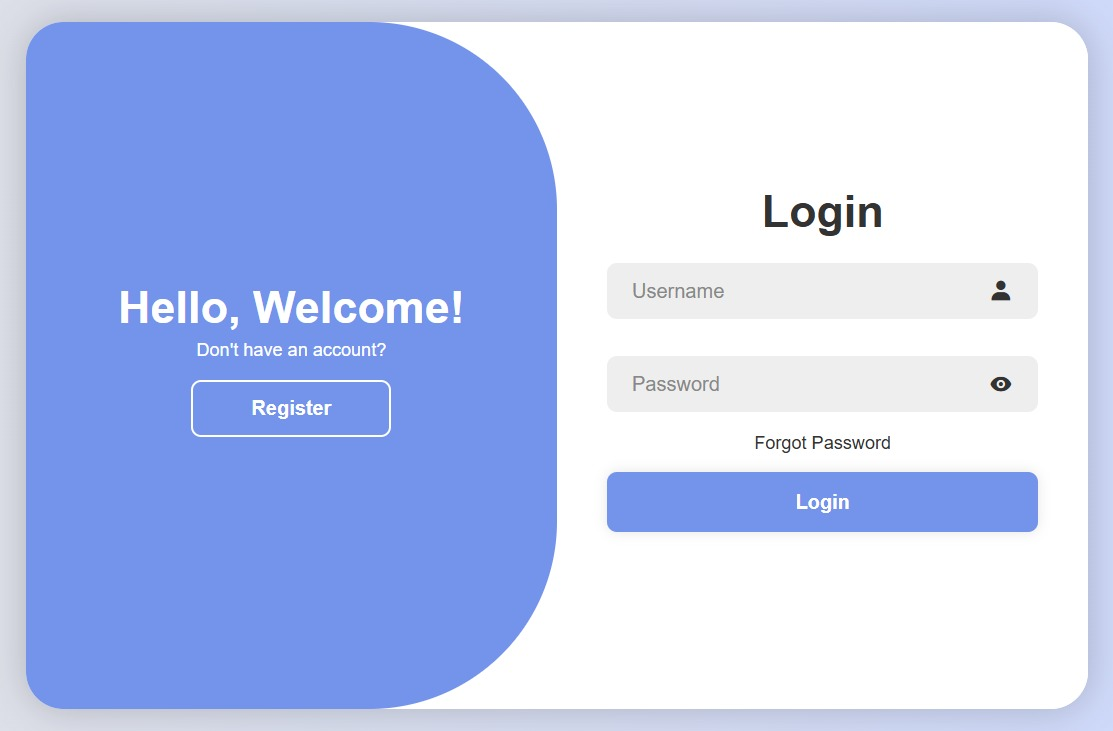
\includegraphics[width=\linewidth]{6/login.jpg}
        \captionof{figure}{Company Login Page}
    \end{minipage}
    \hfill
    \begin{minipage}{0.45\textwidth}
        \centering
        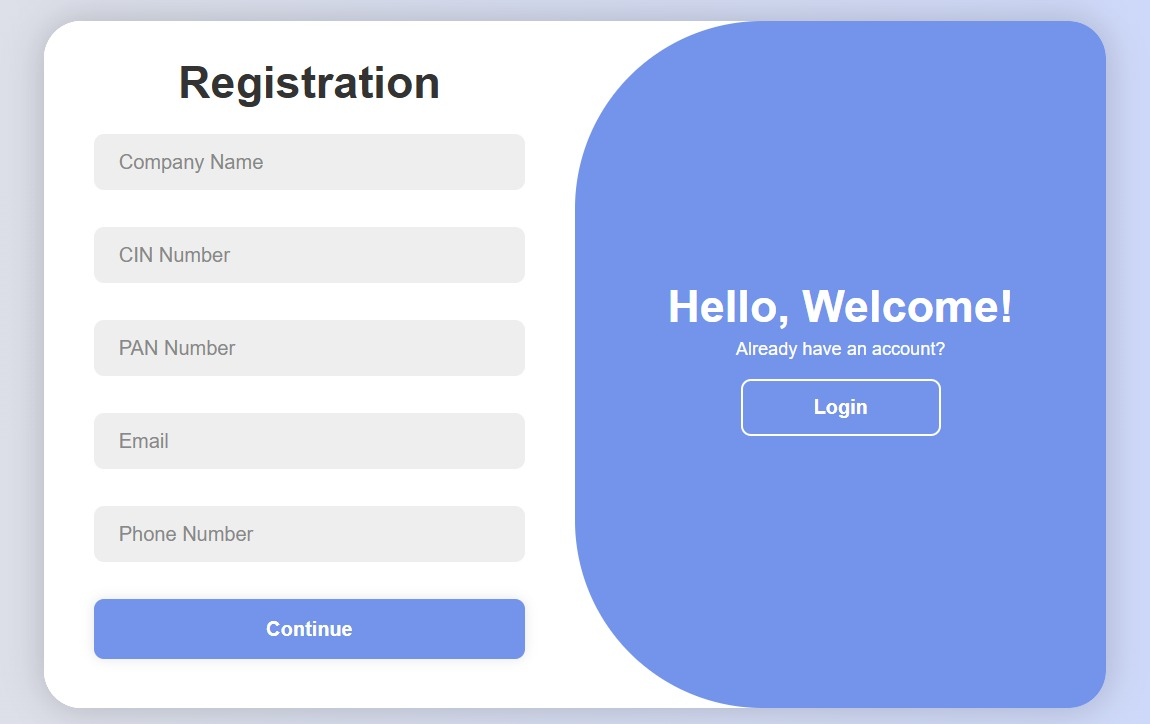
\includegraphics[width=\linewidth]{6/registration.jpg}
        \captionof{figure}{Company Registration Page}
    \end{minipage}
    
    \vspace{1cm} % Adds space before the third image
    
    \begin{minipage}{0.3\textwidth}  % Adjusted width for consistency
        \centering
        \includegraphics[width=\linewidth]{6/Mobile_login.jpg}
        \captionof{figure}{Delivery Personnel Page}
    \end{minipage}
\end{center}
\subsection{Package \& Employee Details Page}
Package Details: Displays information about uploaded packages, including destination, weight and qr code ensuring efficient assignment.
\\
Employee Details: Lists registered employees with availability status, allowing companies to allocate deliveries effectively.
\begin{center}
    \begin{minipage}{0.45\textwidth}
        \centering
        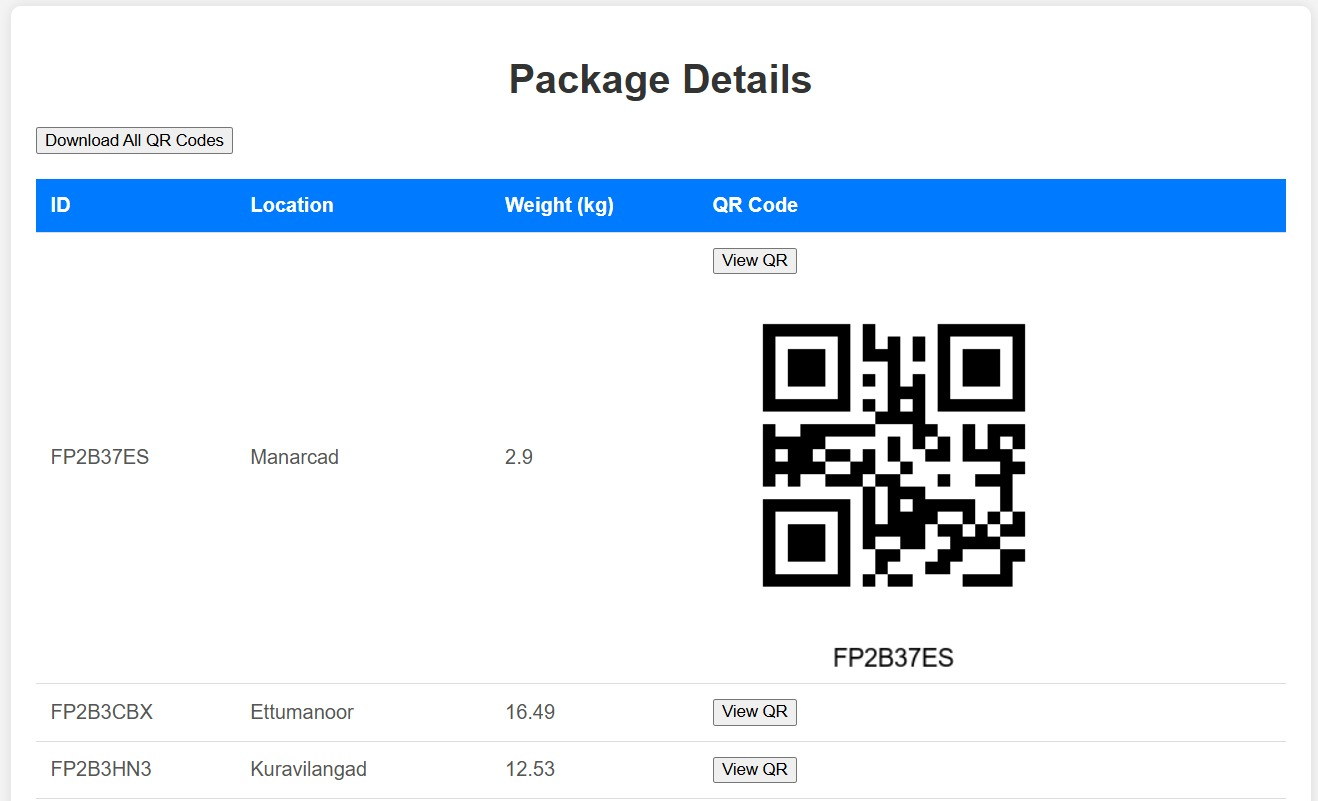
\includegraphics[width=\linewidth]{6/package_details.jpg}
        \captionof{figure}{Package Details Page}
    \end{minipage}
    \hfill
    \begin{minipage}{0.45\textwidth}
        \centering
        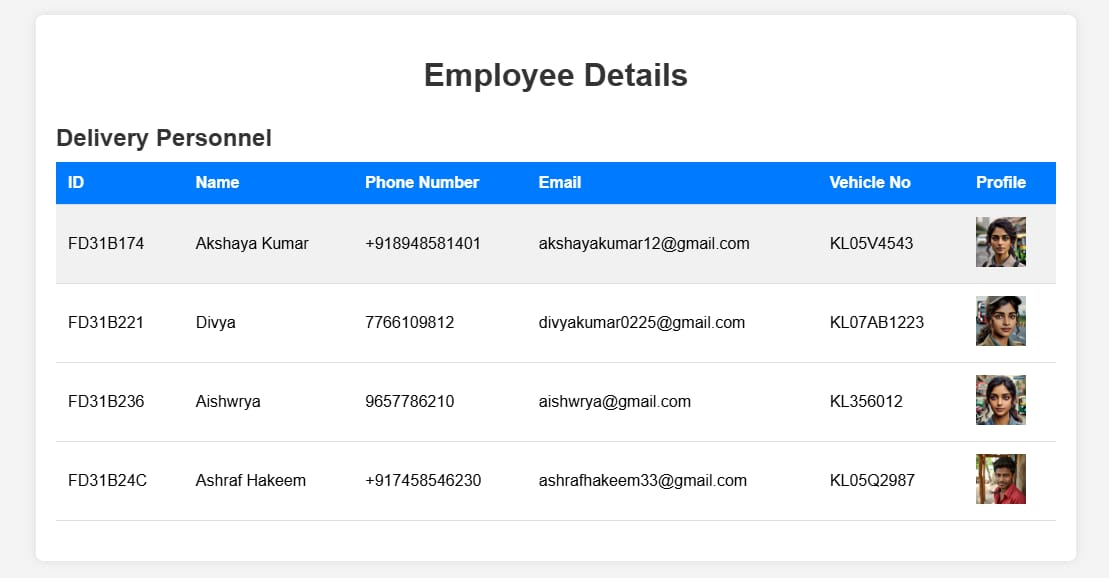
\includegraphics[width=\linewidth]{6/employee_details.jpg}
        \captionof{figure}{Employee Details Page}
    \end{minipage}
\end{center}
\subsection{QR Code Scanning Page}
The system enables companies to generate QR codes for packages, allowing employees to scan them for quick retrieval of delivery details. This feature ensures efficient tracking, reduces manual errors and enhances the overall package management process.

\begin{figure}[H]
\centering
\begin{minipage}{0.24\textwidth}
    \centering
    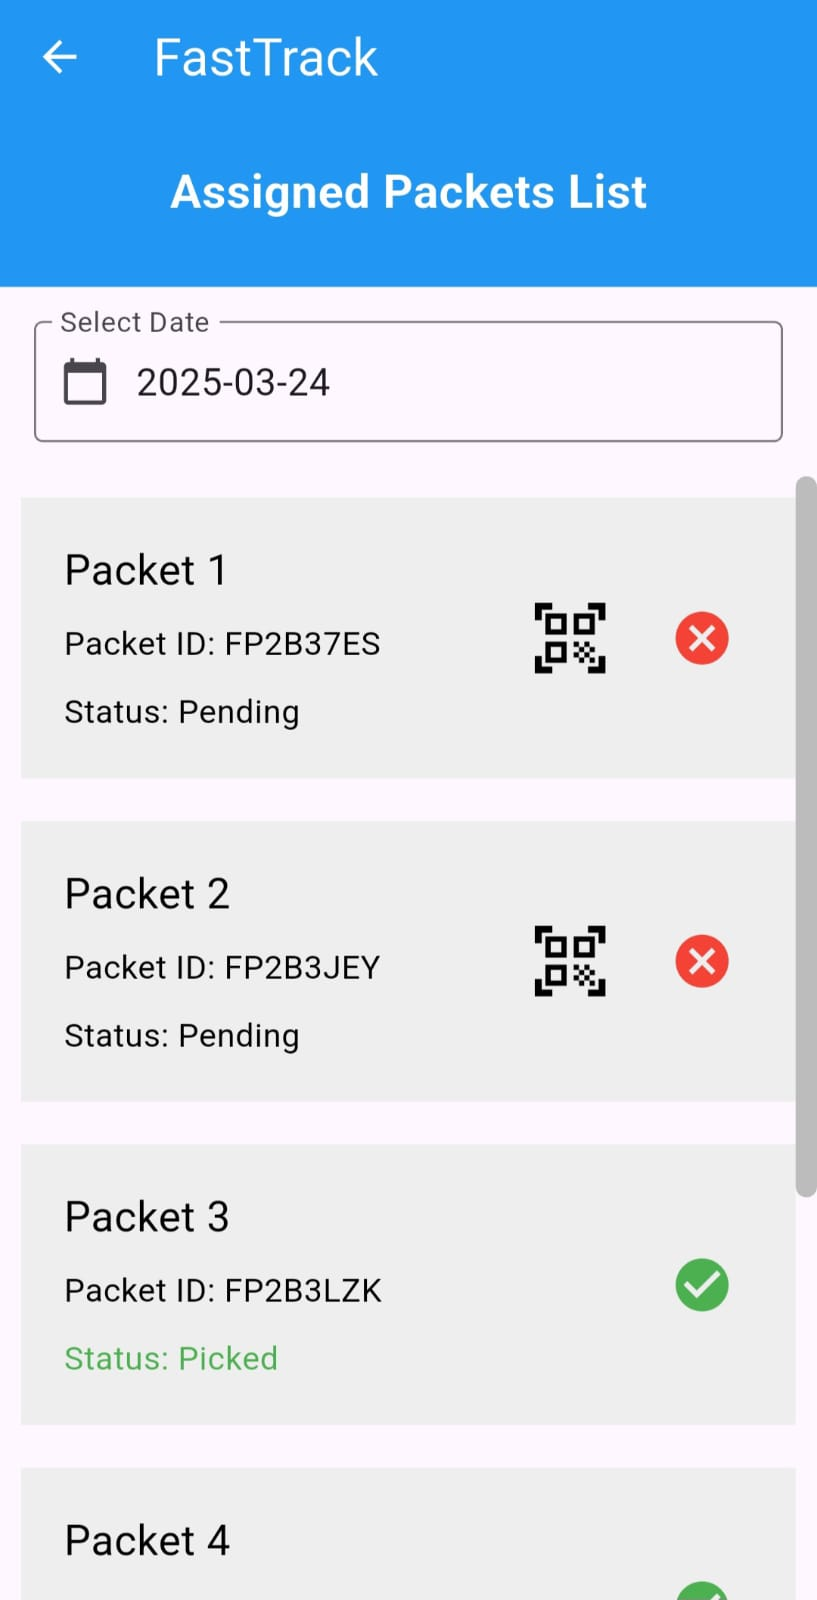
\includegraphics[width=\linewidth]{6/qr1.jpg}
    \label{fig:qr1}
\end{minipage}%
\hspace{5mm}
\begin{minipage}{0.24\textwidth}
    \centering
    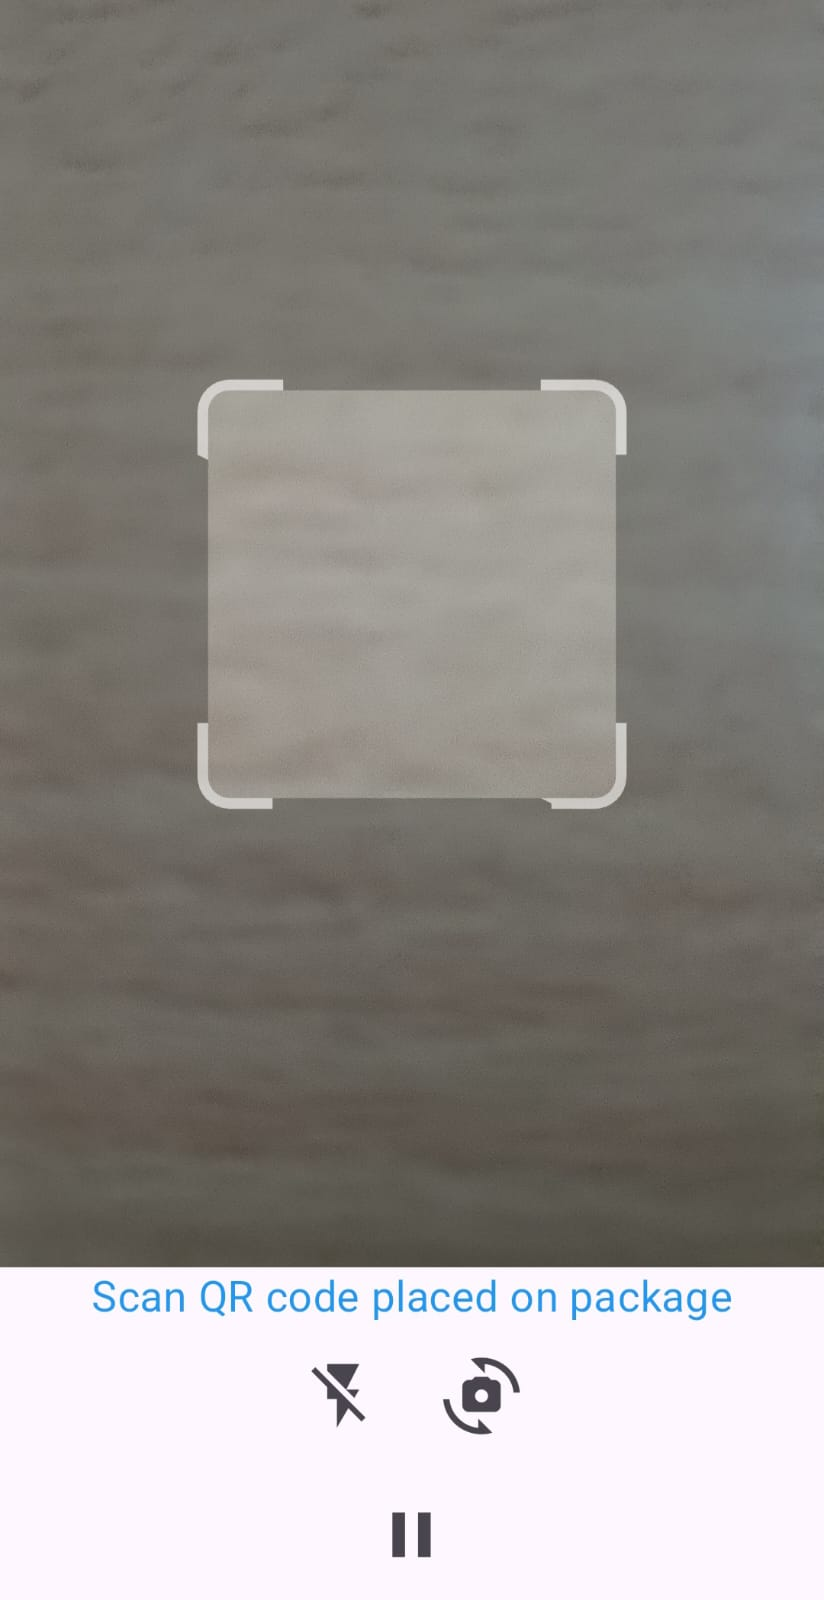
\includegraphics[width=\linewidth]{6/qr2.jpg}
    \label{fig:qr2}
\end{minipage}
\caption{QR Code Scanning}
\label{fig:qrcodes1}
\end{figure}
\subsection{Route Optimization \& Navigation Page}
Route Optimization: Utilizes the Greedy Algorithm and Google Maps API to calculate the efficient delivery routes, minimizing travel distance and time.
\\
Navigation Page: Provides real-time tracking for delivery personnel, ensuring smooth and timely deliveries.
\begin{figure}[H]
\centering
\begin{minipage}{0.24\textwidth}
    \centering
    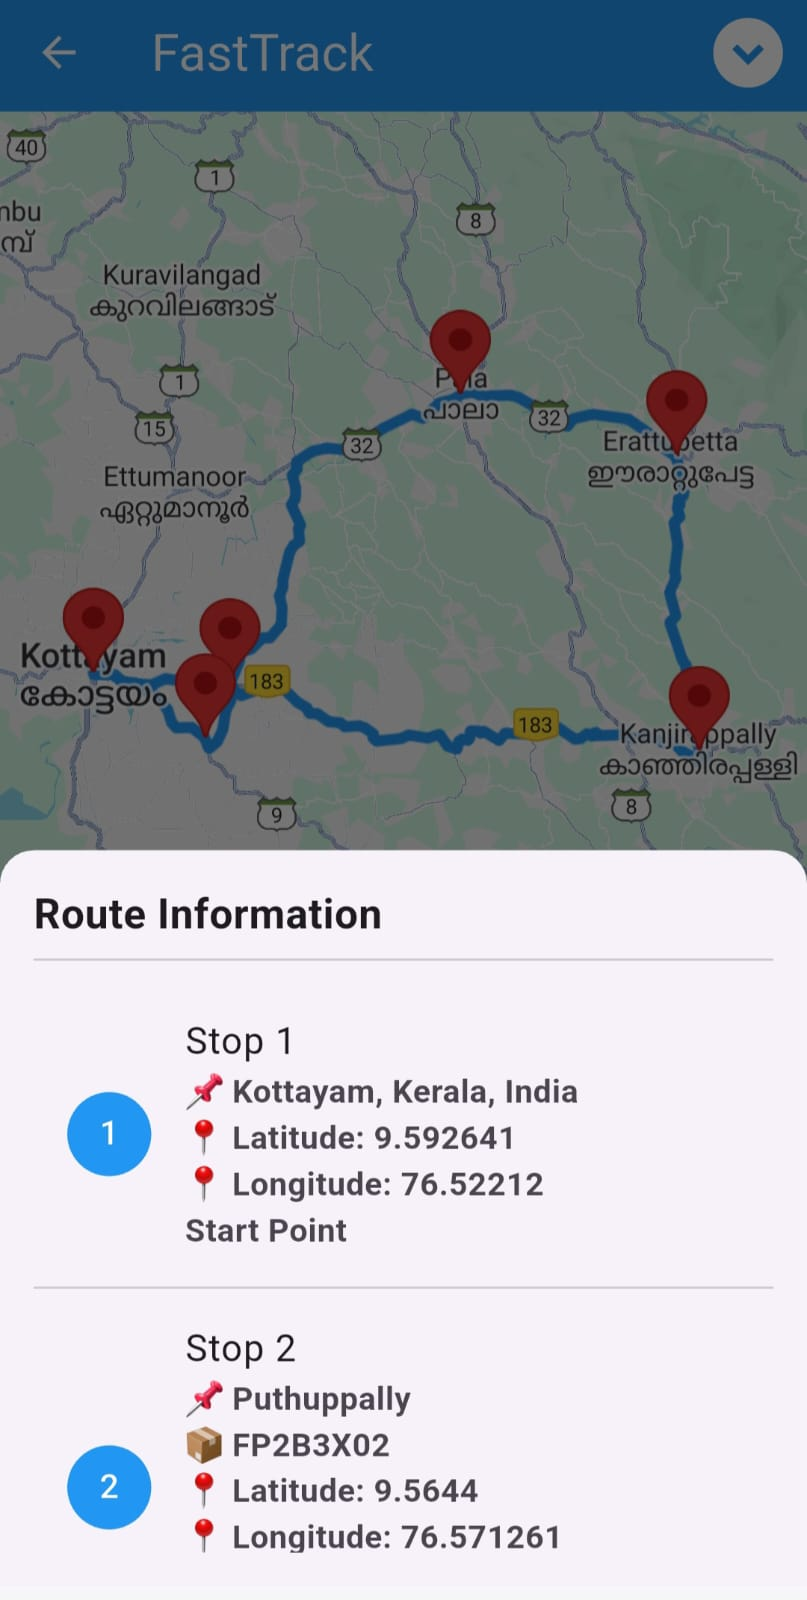
\includegraphics[width=\linewidth]{4/Route_Optimization2.jpg}
    \label{fig:route_optimization26}
\end{minipage}%
\hspace{5mm}
\begin{minipage}{0.24\textwidth}
    \centering
    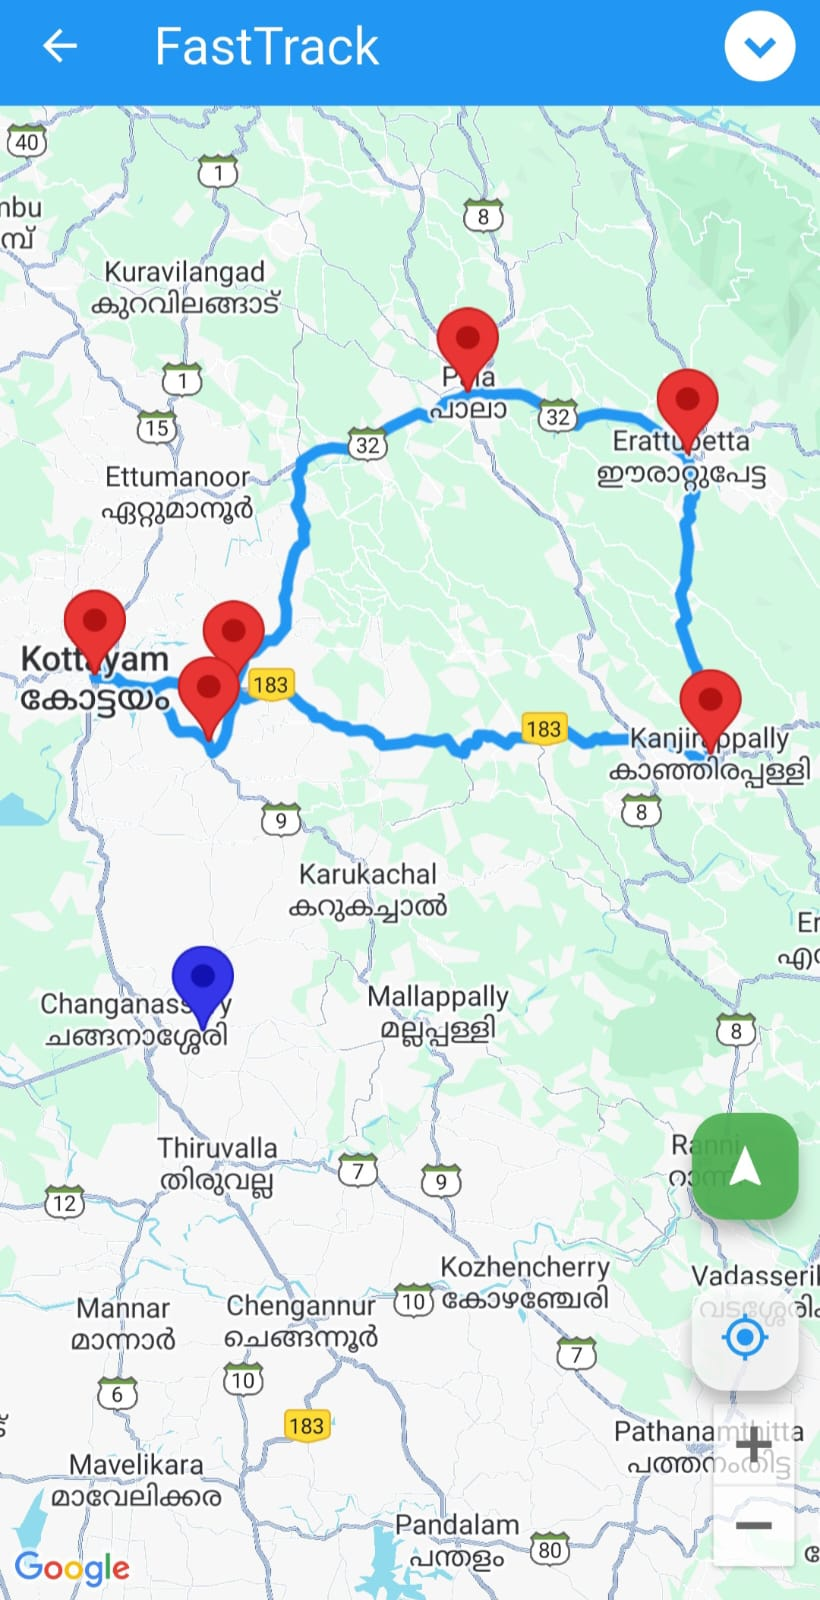
\includegraphics[width=\linewidth]{4/Route_Optimization1.jpg}
    \label{fig:route_optimization16}
\end{minipage}
\caption{Route Optimization and Navigation Page}
\label{fig:route_optimization_combined1}
\end{figure}
\section{Performance Analysis}
The main two algorithms we make use in our project are package assignment and route optimization (Greedy Algorithm). 
% Package Assignment Efficiency Graph
\begin{figure}[h]
    \centering
    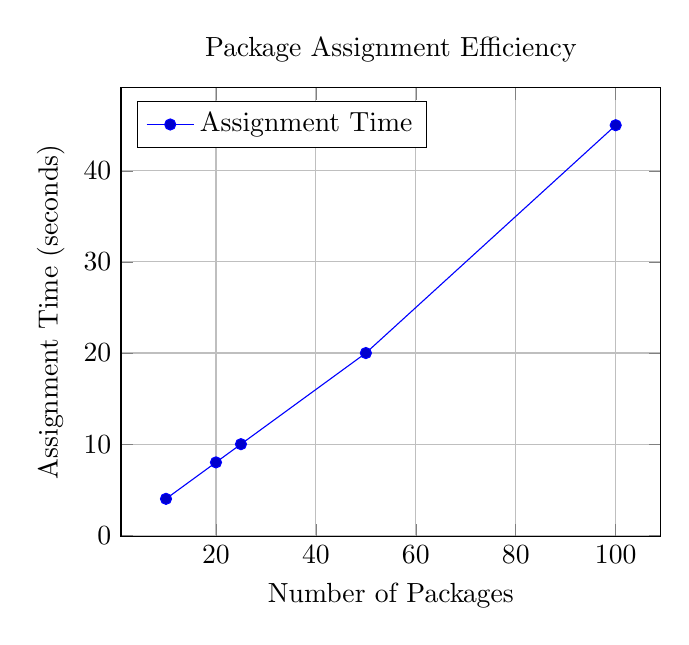
\begin{tikzpicture}
        \begin{axis}[
            title={Package Assignment Efficiency},
            xlabel={Number of Packages},
            ylabel={Assignment Time (seconds)},
            legend pos=north west,
            grid=major
        ]
        \addplot coordinates {(10,4) (20, 8) (25,10) (50,20) (100,45)};
        \addlegendentry{Assignment Time}
        \end{axis}
    \end{tikzpicture}
    \caption{Package Assignment Efficiency Analysis}
\end{figure}

% Route Optimization Performance Graph
\begin{figure}[h]
    \centering
    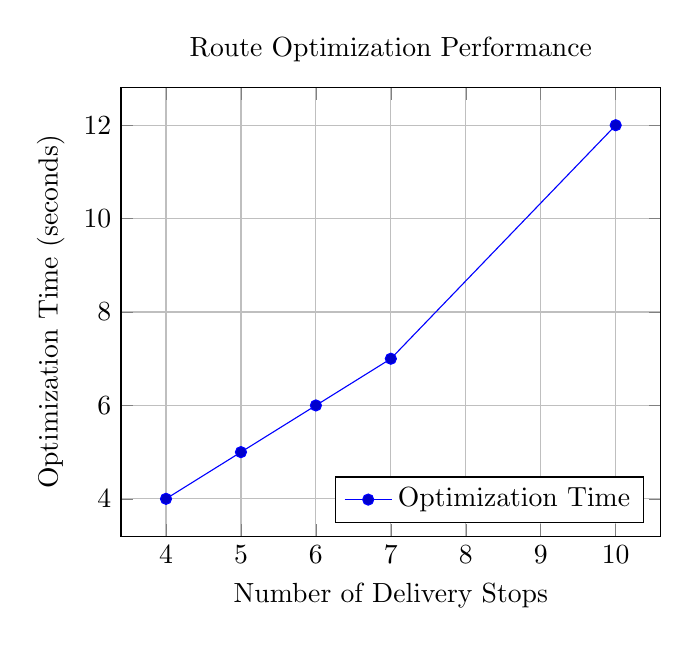
\begin{tikzpicture}
        \begin{axis}[
            title={Route Optimization Performance},
            xlabel={Number of Delivery Stops},
            ylabel={Optimization Time (seconds)},
            legend pos=south east,
            grid=major
        ]
        \addplot coordinates {(4,4) (5,5) (6,6) (7,7) (10,12)};
        \addlegendentry{Optimization Time}
        \end{axis}
    \end{tikzpicture}
    \caption{Route Optimization Performance Analysis}
\end{figure}
\section{Challenges Faced and Solution}
\subsection{Package Assignment}
\begin{itemize}
    \item Problem: The initial employee assignment algorithm only considered the total weight of packages and the vehicle’s average weight capacity. This approach often led to miscalculations, as it did not account for package size constraints or variations in real-world loading conditions. As a result, even when sufficient employees were assigned, some packages were left undelivered due to improper space utilization. Additionally, the system sometimes suggested more employees than necessary, leading to inefficiencies in workforce allocation.

    \item Solution: The algorithm was improved to factor in both weight and size constraints when calculating the required number of employees. Instead of relying solely on weight-based allocation, the system now calculates employee requirements based on both total weight and total volume.Additionally, package assignments were refined to distribute loads evenly across employees, preventing scenarios where small gaps in available space led to undelivered packages. This enhancement ensures that all packages are assigned efficiently while optimizing the use of available employees and transportation capacity.
\end{itemize}
\subsection{Route Optimization}
\begin{itemize}
    \item Problem: The algorithm did not account for the final delivery location, which resulted in incomplete routes and inefficient navigation. This caused potential delays and suboptimal travel sequences for delivery personnel.
    \item Solution: The routing algorithm was refined to ensure that the final delivery location was always included as a required stop. Additionally, the logic was adjusted to dynamically optimize the route while considering real-time location changes, enhancing delivery efficiency and accuracy.
\end{itemize}
\section{Summary}
This chapter presents the results of the FastTrack system, highlighting key features and performance
analysis. The Login \& Registration Page ensures secure authentication for companies and employees
using Firebase (Figure 6.1 \& 6.2 \& 6.3). The Package \& Employee Details Page displays package
information and employee availability for efficient assignment (Figure 6.4 \& 6.5). A QR Code
Scanning Page allows employees to scan package QR codes for quick tracking and retrieval (Figure
6.6). The Route Optimization \& Navigation Page utilizes the Greedy Algorithm and Google Maps
API to generate efficient delivery routes (Figure 6.7). Performance analysis graphs show package
assignment efficiency and route optimization time, proving the system’s effectiveness (Figure 6.8 \&  6.9). Challenges, such as missing final delivery locations in routing, were resolved by refining the algorithm for accurate navigation and optimal travel sequences.
\chapter{Conclusion and Future Scope}
\label{conclusion}

% Conclusion & Future Scope
\section{Summary}
This project, titled "FastTrack," is designed to enhance delivery efficiency through package assignment and route optimization system. The primary objectives were to develop a dynamic personnel allocation system, ensure timely deliveries and optimize routes in real-time. The system consists of a Flutter-based mobile application and a Flask backend, integrating Firebase Firestore for real-time data synchronization.
\\
The study of system requirements involved defining both functional and non-functional needs, emphasizing user interaction features such as real-time route tracking and push notifications. Performance benchmarks, including response time and GPS accuracy, were considered to ensure smooth operations. The development process followed a structured Software Development Life Cycle (SDLC), incorporating core modules like authentication, route optimization and package assignment. Various algorithms were implemented to optimize the delivery workflow.
\\
The system was built using Flutter for the mobile app, Flask for the backend, and Firebase for cloud storage. Key features include a login system, splash screen, map browsing with Google Maps, real-time navigation updates, and Firebase notifications. The integration of these technologies ensures seamless data flow between delivery personnel and companies.
\\
Comprehensive testing strategies, including Unit Testing, Integration Testing and Black Box Testing, were conducted to validate system performance. Key functionalities, such as location tracking, route optimization, and package assignment, were rigorously tested to ensure reliability and accuracy.
\\
The project successfully meets its objectives by minimizing delivery delays, optimizing workforce utilization and improving last-mile delivery operations. The mobile application enables delivery personnel to dynamically access assigned routes, while companies efficiently manage operations through an interactive web portal. Real-time navigation, Firebase notifications and route optimization contribute to a more efficient and streamlined delivery process.
\\
This report comprehensively documents the development, testing, and results of the FastTrack Delivery project, demonstrating its effectiveness in achieving its goals.
\section{Recommendations for Future Work}
To enhance FastTrack's functionality, usability and efficiency, consider the following improvements:
\begin{enumerate}
    \item Algorithm Enhancements: Explore advanced algorithms for package assignment and route optimization to improve efficiency and accuracy, leveraging AI and real-time data.
    \item User Interface Refinement: Conduct user testing to refine the web and mobile UI, improving usability, accessibility and seamless interaction for businesses and employees.
    \item Performance Optimization: Optimize system performance for faster package processing, real-time route updates and efficient data handling, ensuring smooth operations even with high package volumes.
\end{enumerate}


%------------------------Here include the appendix if required-------------------------------------------------
\appendix
\addcontentsline{toc}{part}{Software Requirements Specification}
% \hspace{10pt}
% \vspace{-200pt}
\appendix
\renewcommand{\thesection}{A.\arabic{section}}
\begin{center}
    \Huge \textbf{Appendix A} \\[5pt]
    \Huge \textbf{Software Requirement Specification}
\end{center}
\section{Introduction}
\subsection{Purpose}
This Software Requirements Specification document outlines the requirements for the FastTrack application, a platform designed to calculate and optimize delivery routes for delivery personnel efficiently. It specifies the functionalities, features, and requirements of the product. It covers aspects like location input, default location integration, route optimization algorithms, time estimation, and route visualization through an interactive map interface.  
The primary scope is to enhance the efficiency and reliability of delivery operations while minimizing travel time and fuel consumption. The application aims to provide an intuitive interface, seamless navigation, and support for real-time updates to improve delivery service quality and customer satisfaction.
\subsection{Document Conventions}

\begin{itemize}
    \item This document follows a standardized format, including numbered sections, bullet points, diagrams, and tables for clarity and readability.
    \item Acronyms, abbreviations, and technical terms are defined upon first usage and compiled in the glossary (Appendix A) for quick reference.
    \item All requirements are assigned unique identifiers and listed systematically to ensure easy tracking and cross-referencing throughout the document. 
\end{itemize}

\subsection{Intended Audience and Reading Suggestions}
This document is intended for the following readers:
\begin{itemize}
    \item Developers: To understand the technical requirements and system functionality.
    \item Project Managers: To track progress and ensure the requirements are implemented.
    \item Testers: To create test cases based on requirements.
    \item End Users (Delivery Personnel and Administrators): To comprehend the application's functionality and benefits.
\end{itemize}

Reading Suggestions include
\begin{itemize}
    \item Overview Sections: Recommended for all readers to gain a general understanding of the application.
    \item Functional and Non-functional Requirements: Crucial for developers, testers, and project managers to ensure proper implementation and verification of the system.
    \item User Interface and Workflow Sections: Important for end users to familiarize themselves with the application's features and usage.
\end{itemize}
\subsection{Project Scope}

The FastTrack application is designed to streamline delivery operations by optimizing routes for delivery personnel. Its key objectives include:
\begin{itemize}
    \item Efficient Route Optimization: Calculating the most efficient delivery route for multiple destinations using advanced algorithms, reducing travel time and fuel consumption.
    \item Default Location Integration: Incorporating a fixed starting point for consistent and reliable route planning.
    \item Interactive Map Visualization: Providing clear and user-friendly route displays, along with real-time navigation support.
    \item Time and Distance Estimation: Offering accurate estimates for delivery time and travel distance to enhance scheduling and customer satisfaction.
    \item Dynamic Updates: Allowing for real-time adjustments to routes in response to changes, such as additional stops or delays.
\end{itemize}
The application aims to improve delivery efficiency, reduce operational costs, and ensure timely deliveries while enhancing the overall user experience for delivery personnel and service providers.

\subsection{References}

\begin{itemize}
    \item Route Optimization Apps to Minimize Delivery Delays with Dynamic Routes, nandbox, 2024. Retrieved from nandbox.com
    \item Route4Me API and SDK Developer Documentation, Route4Me, 2024. Retrieved from support.route4me.com
    \item How to Use Python for Route Optimization in Logistics, Data Head Hunters Academy, 2024. Retrieved from dataheadhunters.com
    \item Delivery Route Optimization in Python, AskPython, 2024. Retrieved from askpython.com
\end{itemize}

\section{Overall Description}
\subsection{Product Perspective}
The FastTrack application is a new, self-contained product designed to address the challenges of delivery route optimization. Unlike existing manual or semi-automated systems, FastTrack leverages advanced algorithms and geolocation technology to create an intuitive, user-friendly platform for delivery personnel.
This application operates independently, without requiring integration with any legacy systems, but can seamlessly integrate with popular GPS and mapping tools. It is designed to serve small and medium-sized businesses seeking efficient delivery solutions, enhancing operational efficiency and reducing delivery time.
The concept stems from the need to simplify delivery operations, reduce costs, and improve the overall reliability of delivery services, particularly in dynamic environments with multiple destination points.
\subsection{Product Features}
The primary feature of FastTrack include:
\begin{enumerate}
    \item Route Optimization: Users can efficiently plan routes with up to 300 stops, utilizing real-time traffic data and delivery-specific parameters for optimized navigation.
    \item Dynamic Route Adjustment: Users can adapt to changing conditions through real-time route adjustments, minimizing delays caused by traffic, road closures, or weather disruptions.
    \item Proof of Delivery and Documentation: Users can securely document proof of delivery through photos, notes, and signatures, ensuring seamless record-keeping and dispute resolution.
    \item Dynamic Data-Driven Delivery Insights: Users can access detailed delivery performance insights, including metrics like distance, time, and fuel savings, with exportable reports for analysis and improvement.
    \item Route Export and Data Integration: The system enables seamless export of route data in CSV or Excel formats, ensuring integration with logistics and operations management systems.
\end{enumerate}

\subsection{User Classes and Characteristics}

\begin{itemize}
    \item Admin: Responsible for overseeing operations, managing user accounts, monitoring system performance, and resolving issues. Requires a moderate to high level of technical expertise and familiarity with system functionalities.
    \item Delivery Personnel: Primarily uses the product for route optimization, proof of delivery, and real-time updates. Requires basic technical expertise and familiarity with smartphone applications.
    \item Technical Expertise: Includes developers and system administrators responsible for maintaining the application, integrating APIs, and ensuring system reliability. Requires advanced technical knowledge and troubleshooting skills.
    \item Company: Refers to stakeholders or management personnel who utilize delivery insights, performance reports, and other analytics for decision-making. Requires a high-level understanding of operational metrics but minimal technical expertise.
\end{itemize}

\subsection{Operating Environment}
\
\begin{itemize}
    \item Hardware Platform:
    \begin{itemize}
        \item Mobile devices with at least 2 GB of RAM and 16 GB of internal storage.
        \item GPS enabled smartphone.
    \end{itemize}
    \item Operating System:
    \begin{itemize}
        \item Android (Version 8.0 and above).
        \item iOS (Version 13.0 and above).
    \end{itemize}
\end{itemize}

\subsection{Design and Implementation Constraints}

\begin{itemize}
    \item Hardware Limitations: Requires smartphones with GPS functionality, a minimum of 2 GB RAM and stable internet connectivity.
    \item Security Considerations: Data exchanged between the app and server will be encrypted using HTTPS for secure communication.
    \item Programming Standards: The application will be developed using modern frameworks like Flutter for cross-platform compatibility.
    \item Database Technology: A cloud-based database, such as Firebase will store route details, delivery data, and user information.
    \item Third-party APIs: Integration with GPS services for route optimization and location tracking.
    \item Design Standards: Adherence to mobile app design conventions for usability and accessibility.
\end{itemize}

\subsection{User Documentation}

The following user documentation components will be delivered with the FastTrack application to ensure ease of use and proper understanding of its features:
\begin{itemize}
    \item User Manual:A comprehensive guide in PDF format that covers installation, setup, usage, troubleshooting, and frequently asked questions.
    \item Online Help: Context-sensitive help integrated within the application, offering quick access to tooltips and feature explanations.
    \item Tutorials: Video tutorials hosted on the app, demonstrating key functionalities like route planning and navigation.
    \item Quick Start Guide: A concise, easy-to-follow document that provides a fast overview of the application’s primary features and setup instructions.
    \item Release Notes: A detailed document that outlines new features, updates, and bug fixes for each version, available in PDF format.
\end{itemize}

\subsection{Assumptions and Dependencies}

Assumptions include:
\begin{itemize}
    \item Users have access to GPS-enabled smartphones with stable internet connectivity.
    \item The application will primarily operate within areas where GPS accuracy and internet speed are reliable.
    \item Delivery routes provided by third-party services are accurate and up-to-date.
\end{itemize}
Dependencies include:
\begin{itemize}
    \item Stable and continuous GPS and internet services for route optimization and real-time updates.
    \item Functional smartphones meeting the specified hardware requirements.
    \item Continued availability and performance of third-party APIs for GPS and location services.
    \item Reliable cloud-based database for storing user data, route details, and delivery updates.
\end{itemize}

\section{System Features}
\subsection{Route Optimization}
\subsubsection{Description and Priority}

\begin{itemize}
    \item Description: Curates the best route from an extensive list of destinations (up to 200 per route) and tailored vehicle types.
    \item Priority: High
    \item Benefit: 9
    \item Penalty: 1
    \item Cost: 8
    \item Risk: 3
\end{itemize}

\subsubsection{Stimulus/Response Sequences}

\begin{itemize}
    \item Stimulus: User inputs a list of destinations.
    \item Response: The system generates the most optimized route based on distance and time, considering current traffic conditions.
\end{itemize}

\subsubsection{Functional Requirements}

\begin{itemize}
    \item The system should be capable of handling up to 300 stops per route without additional cost.
    \item The route should be optimized using real-time traffic data, considering factors such as time, distance, and mode of delivery.
    \item The system should offer quick optimization for routes with up to 100 stops in 5 seconds.
    \item The user should be able to save and duplicate routes, adding new destinations from previous routes easily.
\end{itemize}
	
\subsection{Dynamic Route Adjustment}
\subsubsection{Description and Priority}

\begin{itemize}
    \item Description: Allows dynamic adjustments to routes in real-time based on changing conditions (e.g., traffic, weather, etc.).
    \item Priority: High
    \item Benefit: 9
    \item Penalty: 1
    \item Cost: 7
    \item Risk: 3
\end{itemize}

\subsubsection{Stimulus/Response Sequences}

\begin{itemize}
    \item Stimulus: Real-time data indicates a traffic jam or road closure.
    \item Response: The system automatically adjusts the route to avoid delays, presenting the updated route to the driver.
\end{itemize}

\subsubsection{Functional Requirements}

\begin{itemize}
    \item The system must be capable of adjusting routes in real-time based on live traffic, road closures, and weather conditions.
    \item The system should ensure minimum disruption when adding or removing stops in dynamic routes.
\end{itemize}

\subsection{Proof of Delivery and Documentation}
\subsubsection{Description and Priority}

\begin{itemize}
    \item Description: Captures proof of delivery via photos, notes, and signatures.
    \item Priority: Medium
    \item Benefit: 7
    \item Penalty: 2
    \item Cost: 5
    \item Risk: 3
\end{itemize}

\subsubsection{Stimulus/Response Sequences}

\begin{itemize}
    \item Stimulus: User completes a delivery.
    \item Response: The system captures proof (photos, notes, or signatures) for documentation purposes.
\end{itemize}

\subsubsection{Functional Requirements}

\begin{itemize}
    \item The system should allow users to capture and save photos, notes, and signatures for each stop as proof of delivery.
    \item It must provide the ability to export this proof for further documentation or dispute resolution.
    \item The system should automatically associate proof of delivery with the corresponding stop for easy access.
\end{itemize}

\subsection{Dynamic Data-Driven Delivery Insights}
\subsubsection{Description and Priority}

\begin{itemize}
    \item Description: Provides detailed statistics on delivery performance, including distance, time, and fuel costs saved.
    \item Priority: Medium
    \item Benefit: 7
    \item Penalty: 4
    \item Cost: 7
    \item Risk: 2
\end{itemize}

\subsubsection{Stimulus/Response Sequences}

\begin{itemize}
    \item Stimulus: User requests a report or insight into delivery performance.
    \item Response: The system generates detailed reports on delivery efficiency, including statistics on time, distance, and fuel costs.
\end{itemize}

\subsubsection{Functional Requirement}

\begin{itemize}
    \item The system should provide detailed performance reports on each delivery, including metrics like distance, time, fuel savings, and ETA accuracy.
    \item It must allow users to access and analyze historical route data for performance improvement
\end{itemize}

\subsection{Route Export and Data Integration}
\subsubsection{Description and Priority}

\begin{itemize}
    \item Description: Facilitates exporting routes in CSV or Excel formats, ensuring compatibility with other systems.
    \item Priority: Medium
    \item Benefit: 7
    \item Penalty: 3
    \item Cost: 6
    \item Risk: 2
\end{itemize}

\subsubsection{Stimulus/Response Sequences}

\begin{itemize}
    \item Stimulus: User requests an export of the current route data.
    \item Response: The system generates the export in CSV or Excel format for integration with other systems.
\end{itemize}

\subsubsection{Functional Requirements}

\begin{itemize}
    \item The system should support exporting route data in CSV and Excel formats.
    \item It must ensure compatibility with other logistics and operations management systems.
    \item The export should include all relevant stop data such as addresses, times, phone numbers, and other custom fields.
\end{itemize}

\section{External Interface Requirements}
\subsection{User Interfaces}

The FastTrack application provides multiple user interfaces to facilitate interactions with the system. The application will feature for mobile interface. Below are the logical characteristics for the interfaces between the software and the users.
\begin{itemize}
    \item Login Screen: The login screen will require users to enter credentials (username/email and password) for authentication. A Forgot Password link will also be provided.
    \item Home Screen: The home screen will display a dashboard with an overview of deliveries, available routes, and important notifications. A navigation bar will allow access to different sections such as Route Optimization, Settings, and User Profile.
    \item Route Optimization Screen: This screen will allow users to input delivery destinations and view the optimized route. It will feature a map interface with a Start Navigation button.
    \item Delivery Details Screen: Once a delivery is selected, users will see detailed information about the delivery, such as destination, estimated time of arrival (ETA), and route breakdown.
\end{itemize}

\subsection{Hardware Interfaces}

Device Compatibility: The application will support GPS-enabled smartphones and tablets meeting the following minimum requirements:
\begin{itemize}
    \item RAM: 2 GB or more to ensure smooth operation of the application.
    \item Storage: 16 GB free space to accommodate the app and required data, including maps and route optimization data.
    \item Operating Systems: The application will support Android 8.0 (Oreo) or higher, and iOS 12.0 or higher to ensure compatibility with the latest device features and updates.
\end{itemize}
The mobile devices will connect to the internet via Wi-Fi or cellular networks (3G, 4G, or 5G) to communicate with the backend server for route optimization, delivery updates, and real-time notifications.

\subsection{Software Interfaces}

\begin{itemize}
    \item Operating Systems: Android (version 8.0 or higher) and iOS (version 12.0 or higher).
    \item Cloud-based database: MySQL and Firebase for storing user data and product details.
    \item Third-party APIs: Google Maps API (Android) and Core Location API (iOS) for real-time location tracking and route optimization.
    \item Data exchanged between the app and server  will use JSON format over HTTPS for secure transmission.
\end{itemize}

\subsection{Communications Interfaces}

\begin{itemize}
    \item Communication Protocols: HTTP/HTTPS for secure client-server communication.
    \item Standards and Security: End-to-end encryption for sensitive data.
    \item Error Handling: Notifications for communication failures.
    \item Synchronization and Transfer Rates: Real-time synchronization for auction updates, product availability, and location tracking and Optimized for low-latency data transfer.
\end{itemize}

\section{Other Nonfunctional Requirements}
\subsection{Performance Requirements}

\begin{itemize}
    \item Response Time: The system must calculate the optimal route within 2 seconds for graphs with up to 500 nodes and within 5 seconds for larger graphs (up to 2,000 nodes).
    \item Scalability: The system should handle up to 1,000 simultaneous delivery route calculations without significant performance degradation.
    \item Scalability: The system should handle up to 1,000 simultaneous delivery route calculations without significant performance degradation.
    \item Data Update: Real-time traffic updates, if integrated, must be processed within 10 seconds to adjust route calculations dynamically.
    \item Algorithm Efficiency: The implemented algorithm must operate with a time complexity in the range of \( O(n^2) \) to \( O(n^3) \) for graphs where  n is the number of locations (destinations).
\end{itemize}
\subsection{Safety Requirements}

\begin{itemize}
    \item Data Integrity: Ensure no loss or corruption of delivery location data during input or output processing.
    \item Error Handling: Provide clear error messages for invalid inputs.
    \item Backup and Recovery: Include backup mechanisms to save progress during route calculations, ensuring the system can recover in case of crashes.
    \item Regulatory Compliance: Adhere to any data protection regulations if user or customer data is involved in the system.
\end{itemize}

\subsection{Security Requirements}

\begin{itemize}
    \item Authentication: Require secure login credentials for users accessing the system, especially for systems deployed in enterprise settings.
    \item Privacy: Ensure sensitive data, such as customer addresses or delivery points, is encrypted during transmission and storage.
    \item Access Control: Restrict administrative functionalities to authorized personnel only.
    \item Fraud Prevention: Detect and prevent malicious route manipulations, such as tampering with delivery point data.
\end{itemize}

\subsection{Software Quality Attributes}

\begin{itemize}
    \item Usability: Provide a simple interface for inputting delivery points and configuring preferences.
    \item Modularity: Implement modular code to simplify debugging and future updates, especially for algorithm enhancements.
    \item Localization: Allow the use of local measurement units and integrate localized traffic data sources if real-time updates are used.
    \item Availability: Implement failover mechanisms to maintain functionality in case of minor hardware or software failures.
    \item Adaptability: Provide support for future updates, including the integration of new mapping services, delivery algorithms, or hardware components, with minimal disruption to existing functionality.
\end{itemize}

\section{Other Requirements}
\subsection{Database Requirements}

\begin{itemize}
    \item The system must utilize a relational database management system (RDBMS) to store user data, delivery routes, location information, and performance metrics.
    \item The database schema must be scalable to handle an increasing number of deliveries, users, and data points as the system grows.
\end{itemize}

\subsection{Internationalization Requirements}

\begin{itemize}
    \item Currency and distance units should be configurable according to the user's region.
    \item Date and time formats should be adjustable based on the user's locale to accommodate international users.
\end{itemize}

\subsection{Legal Requirements}

\begin{itemize}
    \item The application should include clear terms and conditions and privacy policies to inform users about data usage and security measures.
    \item The application must comply with data protection regulations such as the General Data Protection Regulation (GDPR) for users within the EU and Data Protection Laws in India (IT Act, 2000) for users within India.
\end{itemize}

\subsection{Backup and Recovery}

\begin{itemize}
    \item The system must include automated daily backups of all critical data, ensuring recovery in the event of data loss or corruption.
    \item A disaster recovery plan should be in place to restore full functionality within 24 hours of a major system failure.
\end{itemize}

\section{Appendix A: Glossary}

\begin{itemize}
    \item API (Application Programming Interface): A set of protocols and tools that allow different software applications to communicate with each other.
    \item GPS (Global Positioning System): A satellite-based navigation system that provides location and time information anywhere on Earth.
    \item RDBMS (Relational Database Management System): A database management system that stores data in a structured format using rows and columns.
    \item Route Optimization: The process of determining the most efficient path or route for delivery based on various factors like distance, time, and traffic.
    \item UI (User Interface): The means by which a user interacts with the system or application, typically through visual elements like buttons, menus, and forms.
    \item API Key: A unique identifier used to authenticate requests to an API service.
    \item ETA (Estimated Time of Arrival): The predicted time a delivery will arrive at a given destination.
    \item GDPR (General Data Protection Regulation): A regulation in the EU law on data protection and privacy in the European Union and the European Economic Area.
    \item Firebase: A platform developed by Google that provides cloud-based backend services like real-time databases, authentication, and hosting for mobile and web applications.
    \item Cloud-based Database: A type of database that is hosted on the cloud, allowing for remote storage and access over the internet.
\end{itemize}

\section{Appendix B: Analysis Models}

\begin{itemize}
    \item Data Flow Diagram (DFD): A diagram showing how data flows through the system. The DFD will include external entities (users, APIs), processes (route optimization, delivery tracking), data stores (delivery data, user profiles), and data flows.
    \item Use Case Diagram: A visual representation of the system's functional requirements, detailing how users (delivery drivers, administrators) will interact with the system (e.g., input destinations, request optimized routes).
    \item Entity-Relationship Diagram (ERD): A diagram that shows the relationships between the different data entities (e.g., Users, Routes, Deliveries, Locations) within the system.
    \item Class Diagram: A diagram that models the object-oriented structure of the system, showing the classes (e.g., User, Route, Delivery) and their relationships.
\end{itemize}


\section{Appendix C: Issues List}
\begin{itemize}
    \item TBD: Integration of third-party APIs: The exact details of integrating the Google Maps API and Core Location API still need to be finalized, including the authentication process and API limits.
    \item Data Synchronization: There is an ongoing discussion about how the real-time delivery updates will synchronize across multiple devices and servers.
    \item Traffic Data Accuracy: Ensuring the accuracy and timeliness of real-time traffic data is a challenge, especially in regions with poor coverage or inconsistent data feeds.
    \item User Interface Design: The exact layout and user flow for the route optimization and delivery tracking screens need further refinement to ensure a seamless user experience.
    \item Security for User Data: The security measures for sensitive user data, especially delivery addresses and contact details, are being reviewed to ensure full compliance with GDPR and other data protection laws.
    \item Device Compatibility Issues: Further testing is required to confirm that the app will function properly across all supported devices, especially for different screen sizes and operating systems.
    \item Route Optimization Algorithm Performance: More tests are needed to ensure the optimization algorithm can efficiently handle large datasets and produce accurate routes in real-time.
\end{itemize}


%-----------------------Here include the references------------------------------------------------------
\nocite{*} 
\bibliographystyle{unsrt}	
\bibliography{references.bib}	
%\cite{cormen2022}
%\cite{swayam2023}
%\cite{makansi2024}
%\cite{workload2024}
%\cite{flutter2024], googlemapsapi, firestore2024, flask2024}
\newpage
\thispagestyle{empty}
\chapter*{Index}
\addcontentsline{toc}{chapter}
{\numberline{}Index}%

     Behavioral Feasibility, 9\\
     Black Box Testing, 36\\
     Detailed Design, 19\\
     Economic Feasibility, 8\\
     Feasibility Study, 8\\
     Functional Requirements, 11\\
     Implementation, 28\\
     Integration Testing, 37\\
     Existing System, 5\\
     Non-Functional Requirements, 11\\
     Proposed System, 6\\
     Requirements Analysis, 10\\
     Requirements Elicitation, 9\\
     Requirements Specification, 10\\
     Requirements Validation, 11\\
     System Design, 13\\
     Technical Feasibility, 9\\
     Testing, 36\\
     Unit Testing, 36\\
     White Box Testing, 37\\


\end{document}
